%!TEX program = xelatex

\documentclass[compress]{beamer}
%--------------------------------------------------------------------------
% Common packages
%--------------------------------------------------------------------------

\definecolor{links}{HTML}{663000}
\hypersetup{colorlinks,linkcolor=,urlcolor=links}

\usepackage[english]{babel}
\usepackage{pgfpages} % required for notes on second screen
\usepackage{graphicx}

\usepackage{multicol}

\usepackage{tabularx,ragged2e}
\usepackage{booktabs}

\setlength{\emergencystretch}{3em}  % prevent overfull lines

\usetheme{hri}
\usetikzlibrary{shapes.geometric}
\usetikzlibrary{svg.path}

% Display the navigation bullet even without subsections
\usepackage{remreset}% tiny package containing just the \@removefromreset command
\makeatletter
\@removefromreset{subsection}{section}
\makeatother
\setcounter{subsection}{1}

\makeatletter
\let\beamer@writeslidentry@miniframeson=\beamer@writeslidentry
\def\beamer@writeslidentry@miniframesoff{%
  \expandafter\beamer@ifempty\expandafter{\beamer@framestartpage}{}% does not happen normally
  {%else
    % removed \addtocontents commands
    \clearpage\beamer@notesactions%
  }
}
\newcommand*{\miniframeson}{\let\beamer@writeslidentry=\beamer@writeslidentry@miniframeson}
\newcommand*{\miniframesoff}{\let\beamer@writeslidentry=\beamer@writeslidentry@miniframesoff}
\makeatother



\newcommand{\source}[2]{{\tiny\it Source: \href{#1}{#2}}}

\usepackage{tikz}
\usetikzlibrary{mindmap,backgrounds,positioning,calc,patterns}

\graphicspath{{figs/}}

\title{Symbolic Reasoning for HRI}
\subtitle{~}
\date{}
\author{Séverin Lemaignan}
\institute{{\bf Bristol Robotics Lab}\\University of the West of England}


% for model of anthopomorphism
\newcommand{\IPA}{{$\mathcal{A}_0$~}}
\newcommand{\SLA}{{$\mathcal{A}_\infty$~}}
\newcommand{\sla}{{\mathcal{A}_\infty}}
\newcommand{\AntMax}{{$\mathcal{A}_{max}$~}}
\newcommand{\antMax}{{\mathcal{A}_{max}}}

% for HATP plans
\newcommand{\hatpaction}[3]{#1\\\textsf{\scriptsize #2,}\\\textsf{\scriptsize #3}}
\newcommand{\stmt}[1]{{\footnotesize \tt  #1}}

% for mutual modelling
\newcommand{\Mmodel}[3]{{\mathcal{M}(#1, #2, #3)}}
\newcommand{\model}[3]{{$\mathcal{M}(#1, #2, #3)$}}
\newcommand{\Model}[3]{{$\mathcal{M}^{\circ}(#1, #2, #3)$}}

% typeset logical concept
\newcommand{\concept}[1]{{\scriptsize \texttt{#1}}}

\begin{document}

\miniframesoff

\licenseframe{github.com/severin-lemaignan/lectures-hri-symbolic-reasoning}

\maketitle

\miniframeson

\begin{frame}{In this lecture}

\begin{itemize}
    \item<1-> Last week: NLP down to syntax parsing
    \item<2-> Today: \textbf{meaning} (both semantics and pragmatics)

    \item<3-> How to attach \emph{meaning} to natural language?
    \item<3-> What are ontologies?
    \item<3-> How is `meaning' represented and used within the robot?
    \item<3-> How does it relate to \emph{mental models}?

\end{itemize}

\end{frame}


\section*{Introduction}


\imageframe{pr2-baby-3}


\begin{frame}[plain]

    \centering
    {\bf Situated dialogue} effectively evidences the challenges

    \begin{columns}
        \begin{column}{0.5\linewidth}
            How can the robot make sense of and act upon a command like:
            \vspace{2em}

            \bf
            ``Can you give me that book?''
        \end{column}
        \begin{column}{0.5\linewidth}
            \begin{center}
                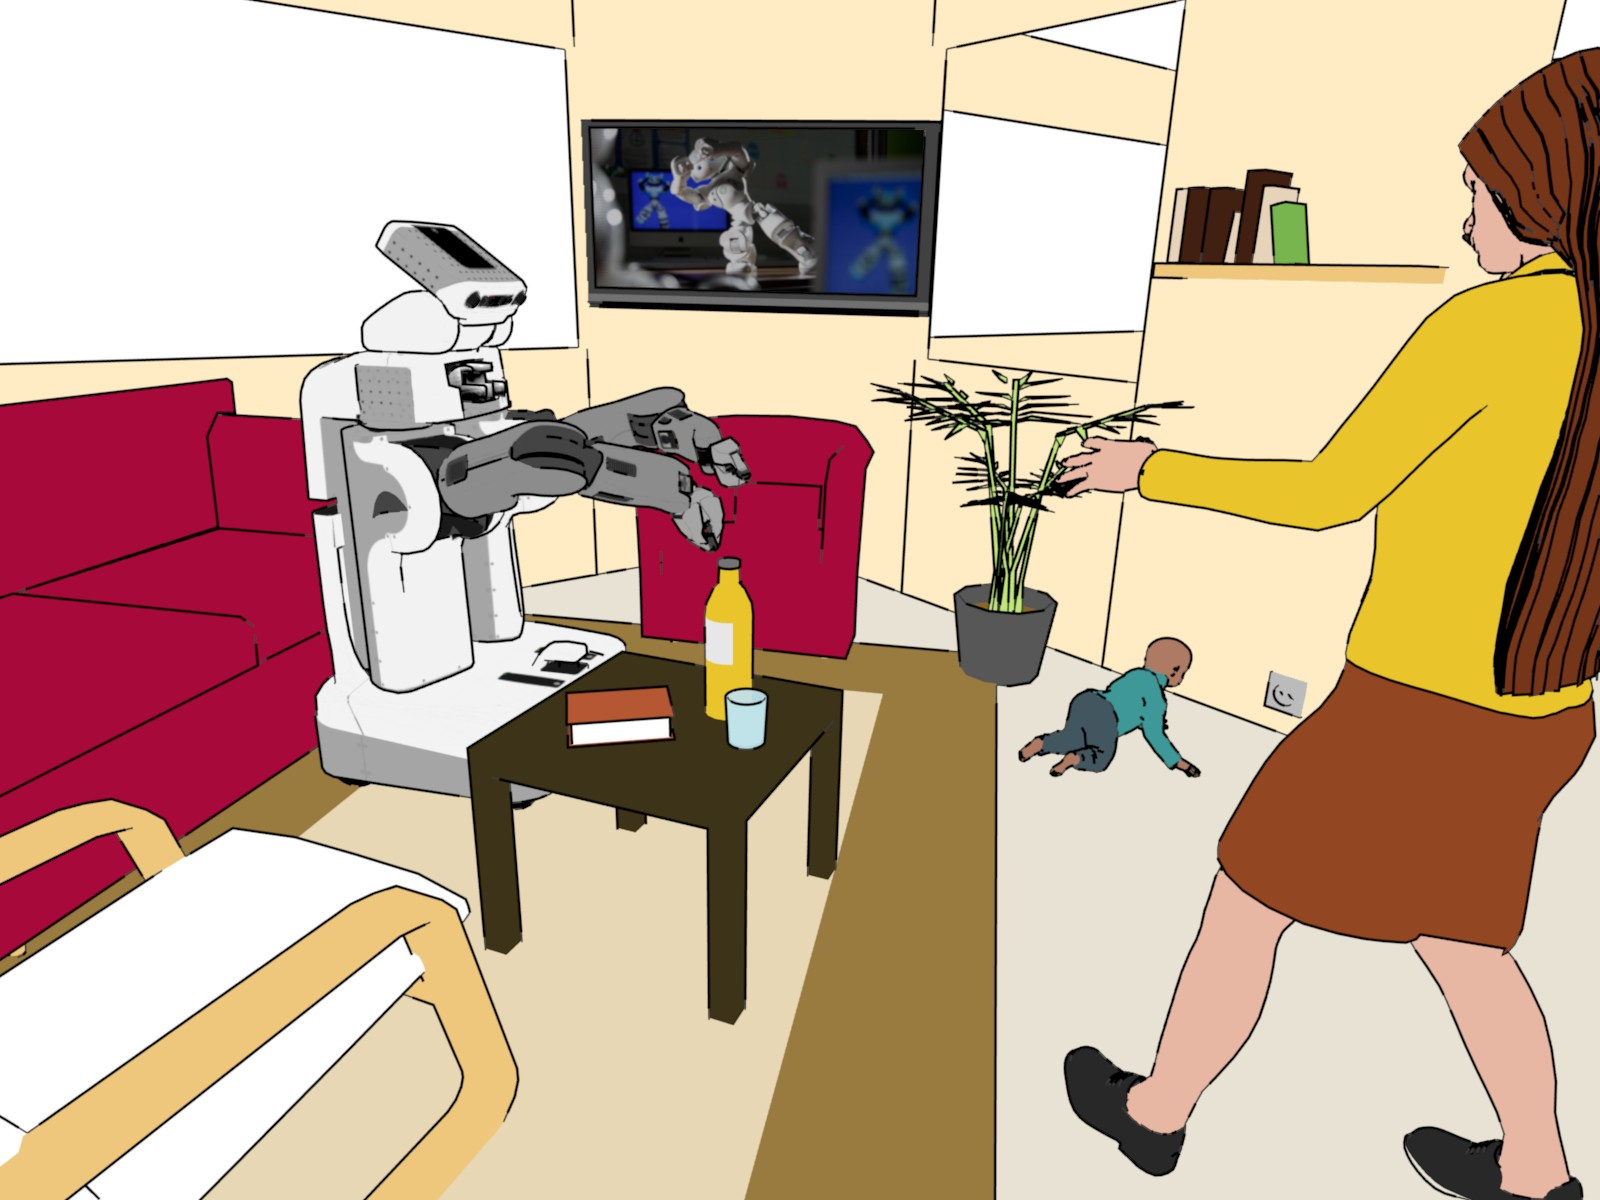
\includegraphics[width=\linewidth]{pr2-baby-3}
            \end{center}
        \end{column}
    \end{columns}

\end{frame}


{\paper{Harnad, \emph{The Symbolic Grounding Problem}, 1990}

\begin{frame}{The Symbol Grounding Problem}
    \centering
    \Large How to attach meaning to a symbol?

    \normalsize

    \only<2>{

        Searle's \textbf{Chinese Room Argument}

        \begin{center}
            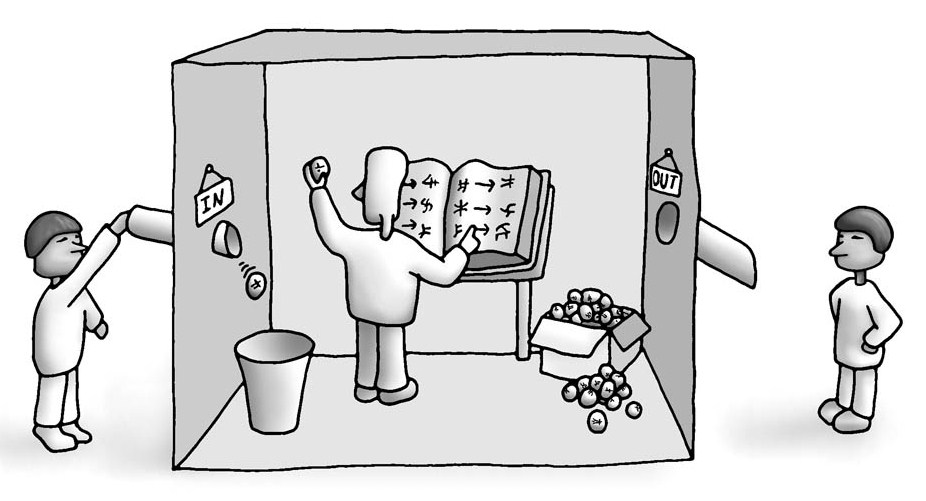
\includegraphics[width=0.8\linewidth]{chinese-room}
        \end{center}


        \href{https://en.wikipedia.org/wiki/Chinese_room}{Read more on Wikipedia}

    }

    \only<3>{

        Is it possible at all?

    }

\end{frame}

}

%%%%%%%%%%%%%%%%%%%%%%%%%%%%%%%%%%%%%%%%%%%%%%%%%%%%%%%%
\section{Symbolic social cognition}


{
    \paper{Lemaignan et al., \emph{Artificial Cognition for Social Human-Robot
    Interaction: An Implementation}, Artifical Intelligence, 2017}
\begin{frame}{Situation Assessment}
        \centering
        \video{0.8\textwidth}{videos/model3d.webm}\\

\end{frame}
}

\begin{frame}{Visual Perspective taking}

        \centering
        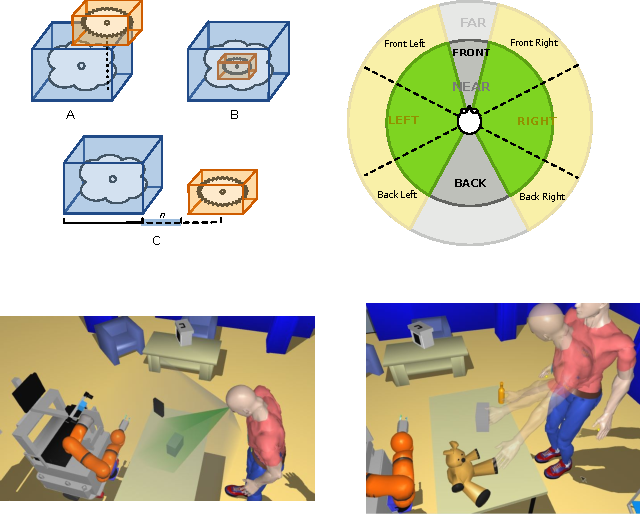
\includegraphics[width=0.8\textwidth]{spark_vert.pdf}

\end{frame}

{
    \paper{Lemaignan et al., \emph{Artificial Cognition for Social Human-Robot
    Interaction: An Implementation}, Artifical Intelligence, 2016}
\begin{frame}{}
        \centering
        \scriptsize

        \begin{tabular}{p{1.5cm}lp{2cm}}
            Subject & Predicate  & Object  \\ 
            \hline
            \concept{Location} & \concept{isAt}  &  \concept{Location}  \\ 
                               &  $\rightarrow$ \concept{isOn}  &   \\ 
                               &  $\rightarrow$ \concept{isIn}  &   \\ 
                               &  $\rightarrow$ \concept{isNextTo}  &   \\ 

            \concept{Location}  & \concept{isAbove}  &  \concept{Location} \\ 
            \concept{Location}  & \concept{isBelow}  & \concept{Location} \\
            \hline
            \concept{Location}  & \concept{hasRelativePosition}  & \concept{Location}  \\ 
                                   & 	$\rightarrow$ \concept{behind} & \\ 
                                      &  $\rightarrow$ \concept{inFrontOf}  & \\ 
                                         &  $\rightarrow$ \concept{leftOf}  &  \\ 
                                            &  $\rightarrow$ \concept{rightOf}  & 	 \\ 
            \concept{Object}  & \concept{farFrom}  &  \concept{Agent} \\ 
            \concept{Object}  & \concept{near}  &  \concept{Agent} \\

            \hline
            \concept{Agent}  & \concept{looksAt}  & \concept{SpatialThing} \\
            \concept{Agent}  & \concept{sees}  &  \concept{SpatialThing}  \\ 
            \concept{SpatialThing}  & \concept{isInFieldOfView}  & \concept{xsd:boolean}  \\ 
            \concept{Agent}  & \concept{pointsAt}  & \concept{SpatialThing} \\ 
            \concept{Agent}  & \concept{focusesOn}  &  \concept{SpatialThing}  \\ 
            \concept{Agent} & \concept{seesWithHeadMovement} &  \concept{SpatialThing} \\
            \concept{Agent} & \concept{canReach} &  \concept{Object} \\ 

        \end{tabular}

\end{frame}
}

{
    \paper{Lemaignan et al. \emph{ORO, a Knowledge Management Module for
    Cognitive Architectures in Robotics}, IROS 2010}
\begin{frame}{From Spatial Model to Symbolic Model}

    \begin{figure}
        \centering

        \resizebox{0.9\paperwidth}{!}{%
            \begin{tikzpicture}[
                    >=latex,
                    every edge/.style={<-, draw, very thick},
                    every node/.style={draw, font=\sf, node distance=0.5, rounded corners,
                align=center, inner sep=5pt,fill=hriSec2Dark!50}]

                \node[fill=hriSec2Comp!50] (thing) {\bf thing};
                \node [fill=hriSec3CompDark!50, node distance=1.8, below left=of thing](sthing) {spatial thing} edge (thing);
                \node [fill=hriSec3CompDark!50, above left=of sthing] {posture} edge (sthing);
                \node [fill=hriSec3CompDark!50, left=of sthing] {shape} edge (sthing);
                \node [fill=hriSec3CompDark!50, below=of sthing] (location) {location} edge (sthing);
                \node [fill=hriSec3CompDark!50, below right=of location] {zone} edge (location);
                \node [fill=hriSec3CompDark!50, below left=of location] (set) {spatial enduring thing} edge (location);
                \node [fill=hriSec3CompDark!50, below right=of set] {obstacle} edge (set);
                \node [fill=hriSec3CompDark!50, below left=of set] {opening} edge (set);
                \node [fill=hriSec3CompDark!50, below=1 of set] {partially tangible thing} edge (set);
                \node [fill=hriSec3CompDark!50, above left=of set] {place} edge (set);

                \node [node distance=1, below right=of thing] (tthing) {temporal thing} edge (thing);
                \node [below=of tthing] (tte) {thing with temporal extent} edge (tthing);
                \node [below right=of tte] {time interval} edge (tte);
                \node [below=1 of tte] (sit) {situation} edge (tte);
                \node [below right=of sit] (evt) {event} edge (sit);
                \node [below right=of evt] (act) {action} edge (evt);
                \node [below=of act] {purposeful action} edge (act);
                \node [below left=of sit] {static situation} edge (sit);

            \end{tikzpicture}
        }

    \end{figure}

\end{frame}
}


\begin{frame}{Ontologies}

    \centering
    \Large
     An \textbf{ontology} encompasses a representation, formal naming, and definition of the categories,
     properties, and relations between the concepts, data, and entities that
     substantiate one, many, or all domains.

     \normalsize

     \onslide<2->{(also known as a \textbf{knowledge graph})}

     \onslide<3>{Ontologies often have close relationships with \textbf{first-order logic
     (FOL)}
     -- more about that later.}

\end{frame}

\begin{frame}{Ontologies}

    \begin{itemize}
        \item \textbf{T-box} statements: the \emph{conceptualisation} of the
            domain, for instance in terms of \emph{categories} (classes): \stmt{Dog
            rdfs:subClassOf Animal}

        \item \textbf{A-box} statements: (T-box compliant) statements about
            \emph{individuals} (instances) in the ontology: \stmt{SPOT rdf:type Dog}

    \end{itemize}

    \pause

    Ontologies are represented using a \textbf{knowledge description} language.
    The \textbf{Web Ontology Langage (OWL)} is a very common choice that uses a
    XML encoding.
\end{frame}

\begin{frame}{Online instanciation}

    \begin{columns}
        \begin{column}{0.4\linewidth}
        \centering
        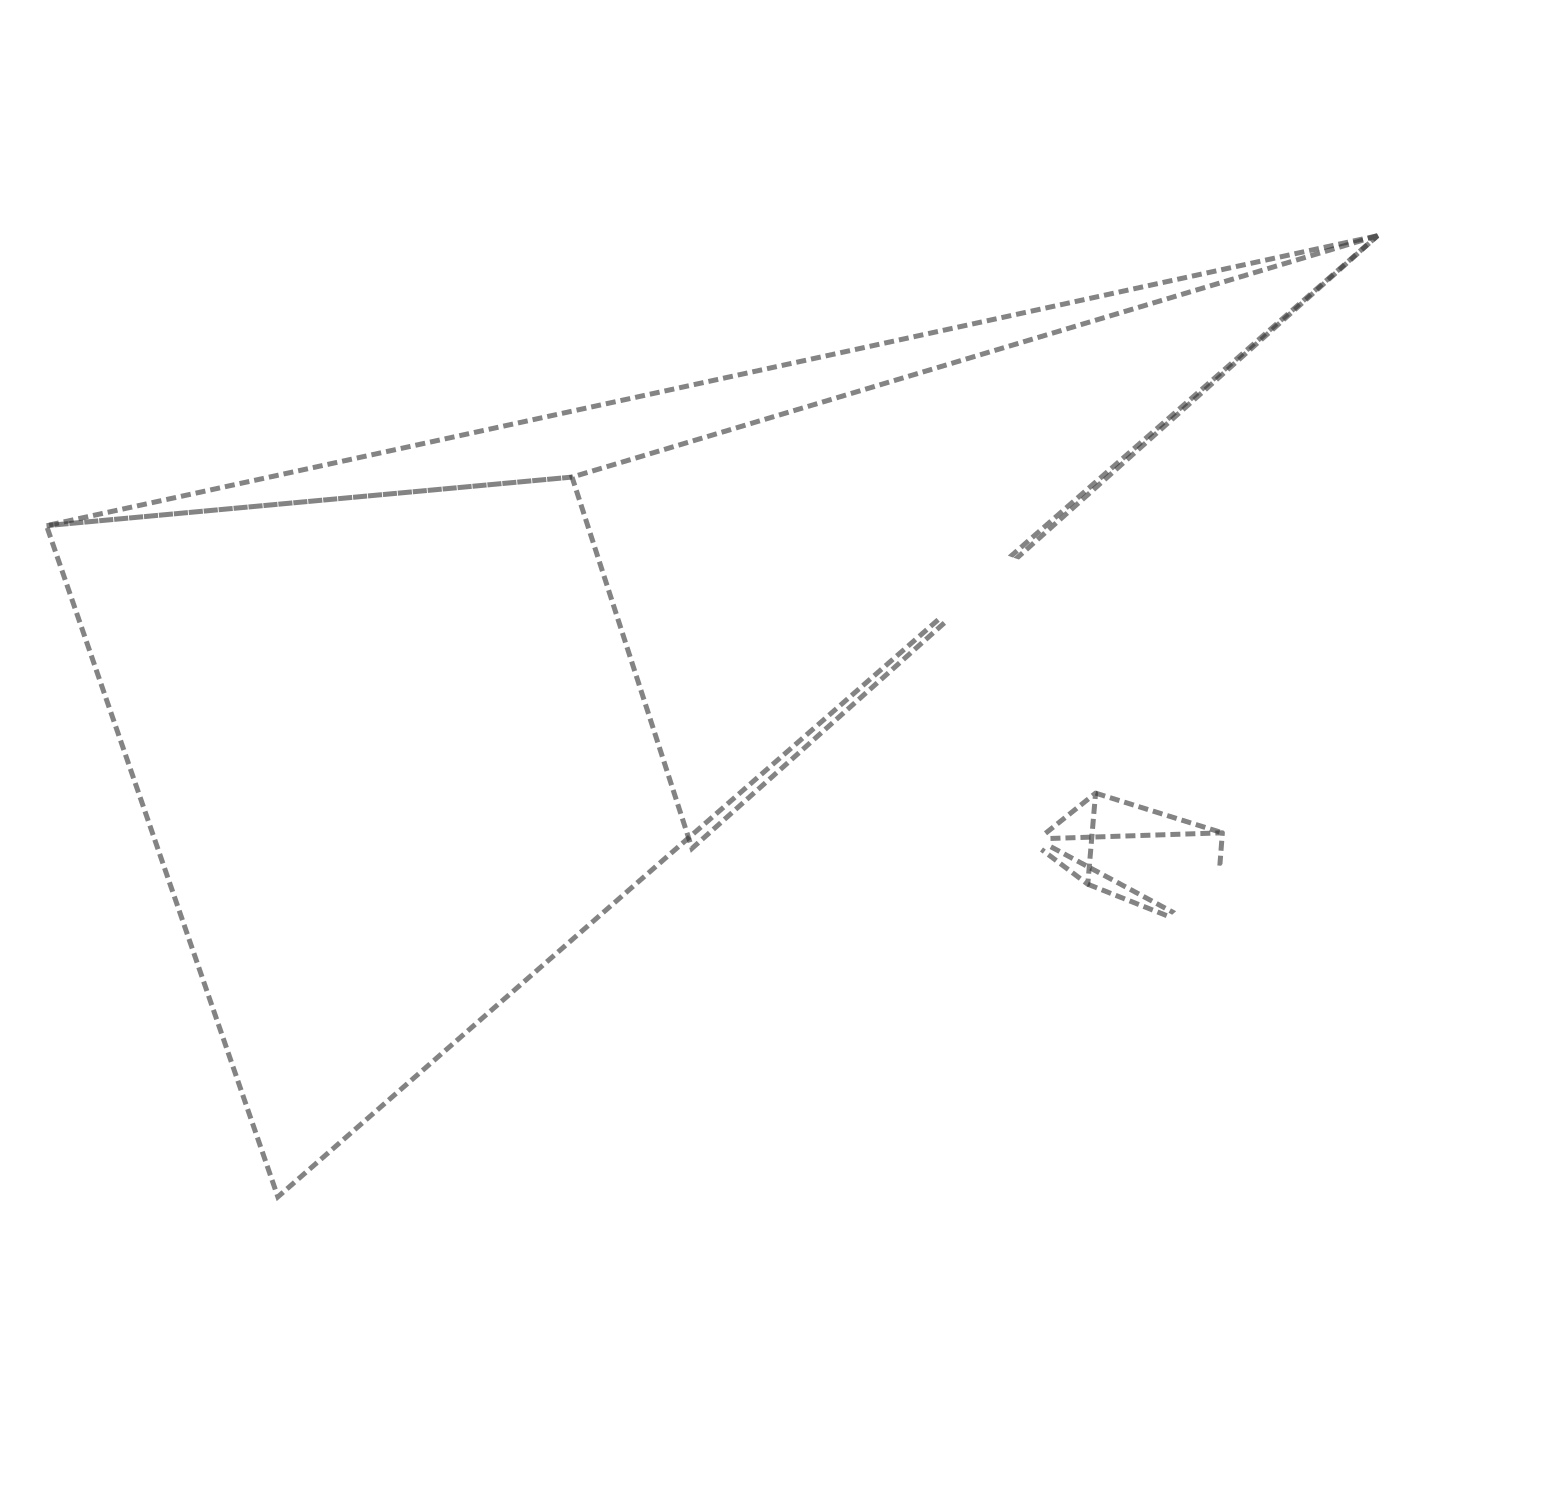
\includegraphics[width=\linewidth]{human-perspective-small}
             
        \end{column}
        \begin{column}{0.6\linewidth}
        
        \begin{figure}

        \resizebox{\columnwidth}{!}{%
        \begin{tikzpicture}[
            yscale=1.3,
            >=latex,
            every edge/.style={<-, draw, very thick},
            every node/.style={draw, font=\sf, node distance=0.5, rounded corners,
            align=center, inner sep=5pt,fill=hriSec2Dark!50},
            classof/.style={<-, draw=black!60, dashed},
            property/.style={<-, draw=hriSec2Comp},
            propname/.style={above, draw=none, fill=none, font=\tt, inner sep=2pt},
            instance/.style={draw=hriSec1Dark, font=\sf, node distance=0.5, rounded corners,
        align=center, inner sep=5pt, fill=none}]

            \node[fill=hriSec2Comp!50] (thing) {\textbf{thing}};
            \node [fill=hriSec3CompDark!50, node distance=1.8, below left=of
            thing](sthing) {place} edge[dashed] (thing);
            \node [fill=hriSec3CompDark!50, below left=of sthing] (agent) {agent} edge (sthing);
                \node [fill=hriSec3CompDark!50, below=of sthing] (artifact) {artifact} edge (sthing);
                \node [fill=hriSec3CompDark!50, below right=of sthing] (location) {physical
                support} edge (sthing);
                \node [fill=hriSec3CompDark!50, below right=of artifact] (table) {table}
                    edge (location) edge (artifact);


            \node [node distance=1, below right=of thing] (tthing) {temporal thing} edge (thing);
                \node [below right=of tthing] (evt) {event} edge[dashed] (tthing);
                            \node [below right=of evt] (act) {action} edge (evt);

        \uncover<2->{
        \draw[dotted, thick] (-8,-3.8) -- +(16, 0);

        \node [instance, below=3 of agent] (human) {human\_1} edge[classof, bend left] (agent);
        \node [instance, above left=of human] (human2) {human\_2} edge[classof, bend left] (agent);
        \node [instance, above right=of human, anchor=south] (robot) {myself} edge[classof, bend left] (agent);
        \node [instance, right=of human, anchor=north west] (book)
            {harry\_potter}
        edge[classof] (artifact);
        \node [instance, right=2 of robot] (ikea) {ikea\_table} edge[classof, bend
        right] (table);
        \node [instance, right=2 of book] (brown) {brown} edge[property] node[propname] {hasColor} (book);


        }
        \uncover<3>{
        \draw[dotted, thick] (-8,-6.2) -- +(16, 0);

        \node [instance, below=5 of act] (moving) {move\_act\_42} edge[classof] (act);
        \path (moving.west) edge [property, out=180, in=-80, looseness=1] node[propname,below] {currentlyPerforms} (human.230);
        \path (human.280) edge [property, out=-80, in=-90, looseness=3.5] node[propname,right] {looksAt} (robot.south);
        \path (ikea.south) edge [property, out=-90, in=-80, looseness=2.5] node[propname, auto] {isOn} (book.320);
        }
        \end{tikzpicture}
        }

        \end{figure}

       \end{column}
    \end{columns}




\end{frame}
%}

%%%%%%%%%%%%%%%%%%%%%%%%%%%%%%%%%%%%%%%%%%%%%%%%%%%%%%%%
%

{
\paper{Lemaignan et al. \emph{Grounding the Interaction: Anchoring
Situated Discourse in Everyday HRI} -- Intl. J. of Social Robotics 2011}

\begin{frame}{Dialogue Grounding}
    \begin{figure}
        \centering

        \resizebox{0.4\paperwidth}{!}{%


            \begin{tikzpicture}[
                    >=latex,
                every edge/.style={draw, very thick},
                skill/.style={draw, rounded corners, align=center, inner sep=5pt, fill=black!20},
                label/.style={midway, align=center, font=\scriptsize, above},
                subpart/.style={rounded corners, draw, align=center, font=\scriptsize, fill opacity=0.5, text opacity=1, fill=white!50}]

            %%% PARSING

            \node at (0,0)[skill, fill=hriSec3CompDark!50] (prepro) {Pre-processing};
                \node [left=0.7 of prepro] (input) {\textbf{Input}};
                \path (input) edge [->] (prepro);

                %\path (spark.100) edge [->, bend right] node[label] {symbolic \\ facts} (oro);
                \node [below =0.4 of prepro, skill, fill=hriSec3CompDark!50] (parsing) {Parsing};
                \path (prepro) edge [->] (parsing);

                \coordinate (base-onto) at (4,0);

                %%% RESOLUTION
                \uncover<2->{
                    \node [below=0.4 of parsing, skill, fill=hriSec3!50, minimum height=4cm, minimum width=5cm] (resolution) {};
                \node [subpart, below=0.2 of resolution.115] (pron) {Pronouns \& \\ anaphora resolution};
                \node [subpart, below=0.2 of pron] (noun) {Noun phrase \\ resolution};
                \node [subpart, right=0.3 of noun, anchor=north west] (discr) {Discrimination};
                \node [subpart, below=0.2 of noun] (verb) {Verbal phrase \\ resolution};
                \node [subpart, cylinder, shape border rotate=90, aspect=0.5, below=0.2 of discr] (actions) {Actions};
                \path (pron) edge [->] (noun);
                \path (noun) edge [->] (discr);
                \path (noun) edge [->] (verb);
                \path (verb) edge [dashed, <->] (actions);
                \path (pron) edge [dashed, <->] node[label] {queries} (pron -| base-onto);
                \path (noun.20) edge [dashed, <->] node[label] {queries} (noun.20 -| base-onto);
                \path (discr) edge [<->] (discr -| base-onto);

                \node [left=0.2 of resolution.west, rotate=90, anchor=south] {Resolution};
                \path (parsing) edge [->] (pron);
            }

            %%% INTERPRETATION
                \uncover<3->{
                    \node [skill, below=0.4 of resolution,minimum width=5cm, minimum height=3cm] (interp) {};
                \node [subpart, below=0.2 of interp.north] (content) {Content analysis};
                \node [below=0.6 of content.south west, subpart] (question) {Question \\ handler};
                \node [below=0.6 of content.south east, subpart] (stat) {Statement \\ builder};
                \path (content) edge [->] node[label, left] {question} (question);
                \path (content) edge [->] node [label, right] {goal | statement} (stat);
                \path (stat) edge [->] node [label] {asserts} (stat -| base-onto);

                \node [left=0.2 of interp.west, rotate=90, anchor=south] {Interpretation};

                \path (verb) edge [->] (content);
                \path (question) edge [dashed, bend right, <->] node[label] {queries} (question.south -| base-onto);
            }

            %%% ONTOLOGY
                \uncover<2->{
                    \node at (resolution.north -| base-onto) [rotate=-90, skill, minimum height=2cm, minimum width=7cm, fill=hriSec3!50, anchor=south west] (onto) {Ontology};

                }

            %%% VERBALIZATION
            \uncover<4->{
                \node [below=0.7 of interp, skill, fill=hriSec2Dark!50] (verb) {Verbalization};
            \path (question) edge [->] (verb);
            \path (stat) edge [->] (verb);
            \path (discr.south east) edge [black!50, dashed, bend left, <->] (verb.north east);
            \node [right=0.7 of verb] (output) {\textbf{Output}};
            \path (verb) edge [->] (output);
        }
        \end{tikzpicture}
        }
    \end{figure}

\end{frame}
}


{
\paper{Lemaignan et al. \emph{Grounding the Interaction: Anchoring
Situated Discourse in Everyday HRI} Intl. J. of Social Robotics 2011}
\begin{frame}{Dialogue Grounding}
    \centering


    \begin{columns}
        \begin{column}{0.65\linewidth}

    \centering
    \vspace*{2em}
    {\bf ``Give me the book on the table''}\\

    \uncover<2-> {
        $\downarrow$\\
        {\tt me} $\rightarrow$ {\tt human\_1} \\
        find({\tt\scriptsize ?obj type table}) $\rightarrow$ {\tt ikea\_table} \\
        find({\tt\scriptsize ?obj type book, ?obj isOn ikea\_table})
        $\rightarrow$ {\tt harry\_potter} \\
    }

    \uncover<3-> {
        $\downarrow$\\
        { \tt
            \textbf{human\_1} desires \textbf{give\_act\_1}, \\
            \textbf{give\_act\_1} type \textbf{Give}, \\
            \textbf{give\_act\_1} performedBy \textbf{myself}, \\
            \textbf{give\_act\_1} actsOnObject \textbf{book}, \\
            \textbf{give\_act\_1} receivedBy \textbf{human\_1} \\
        }
    }
            
        \end{column}
        \begin{column}{0.35\linewidth}
         \resizebox{\linewidth}{!}{%
 
 
             \begin{tikzpicture}[
                     >=latex,
                 every edge/.style={draw, very thick},
                 skill/.style={draw, rounded corners, align=center, inner sep=5pt, fill=black!20},
                 label/.style={midway, align=center, font=\scriptsize, above},
                 subpart/.style={rounded corners, draw, align=center, font=\scriptsize, fill opacity=0.5, text opacity=1, fill=white!50}]
 
             %%% PARSING
 
             \node at (0,0)[skill, fill=hriSec3CompDark!50] (prepro) {Pre-processing};
                 \node [left=0.7 of prepro] (input) {\textbf{Input}};
                 \path (input) edge [->] (prepro);
 
                 %\path (spark.100) edge [->, bend right] node[label] {symbolic \\ facts} (oro);
                 \node [below =0.4 of prepro, skill, fill=hriSec3CompDark!50] (parsing) {Parsing};
                 \path (prepro) edge [->] (parsing);
 
                 \coordinate (base-onto) at (4,0);
 
                 %%% RESOLUTION
                     \node [below=0.4 of parsing, skill, fill=hriSec3!50, minimum height=4cm, minimum width=5cm] (resolution) {};
                 \node [subpart, below=0.2 of resolution.115] (pron) {Pronouns \& \\ anaphora resolution};
                 \node [subpart, below=0.2 of pron] (noun) {Noun phrase \\ resolution};
                 \node [subpart, right=0.3 of noun, anchor=north west] (discr) {Discrimination};
                 \node [subpart, below=0.2 of noun] (verb) {Verbal phrase \\ resolution};
                 \node [subpart, cylinder, shape border rotate=90, aspect=0.5, below=0.2 of discr] (actions) {Actions};
                 \path (pron) edge [->] (noun);
                 \path (noun) edge [->] (discr);
                 \path (noun) edge [->] (verb);
                 \path (verb) edge [dashed, <->] (actions);
                 \path (pron) edge [dashed, <->] node[label] {queries} (pron -| base-onto);
                 \path (noun.20) edge [dashed, <->] node[label] {queries} (noun.20 -| base-onto);
                 \path (discr) edge [<->] (discr -| base-onto);
 
                 \node [left=0.2 of resolution.west, rotate=90, anchor=south] {Resolution};
                 \path (parsing) edge [->] (pron);
 
             %%% INTERPRETATION
                     \node [skill, below=0.4 of resolution,minimum width=5cm, minimum height=3cm] (interp) {};
                 \node [subpart, below=0.2 of interp.north] (content) {Content analysis};
                 \node [below=0.6 of content.south west, subpart] (question) {Question \\ handler};
                 \node [below=0.6 of content.south east, subpart] (stat) {Statement \\ builder};
                 \path (content) edge [->] node[label, left] {question} (question);
                 \path (content) edge [->] node [label, right] {goal | statement} (stat);
                 \path (stat) edge [->] node [label] {asserts} (stat -| base-onto);
 
                 \node [left=0.2 of interp.west, rotate=90, anchor=south] {Interpretation};
 
                 \path (verb) edge [->] (content);
                 \path (question) edge [dashed, bend right, <->] node[label] {queries} (question.south -| base-onto);
 
             %%% ONTOLOGY
                     \node at (resolution.north -| base-onto) [rotate=-90, skill, minimum height=2cm, minimum width=7cm, fill=hriSec3!50, anchor=south west] (onto) {Ontology};
 
 
             %%% VERBALIZATION
                 \node [below=0.7 of interp, skill, fill=hriSec2Dark!50] (verb) {Verbalization};
             \path (question) edge [->] (verb);
             \path (stat) edge [->] (verb);
             \path (discr.south east) edge [black!50, dashed, bend left, <->] (verb.north east);
             \node [right=0.7 of verb] (output) {\textbf{Output}};
             \path (verb) edge [->] (output);
         \end{tikzpicture}
         }

        \end{column}
    \end{columns}


\end{frame}
}
%
%%%%%%%%%%%%%%%%%%%%%%%%%%%%%%%%%%%%%%%%%%%%%%%%%%%%%%%%%

{
    \paper{Lemaignan et al., {\bf Artificial Cognition for Social Human-Robot
    Interaction: An Implementation}, Artifical Intelligence, 2017}
\begin{frame}{Multi-modal interaction}

    \begin{columns}
        \begin{column}{0.4\linewidth}
        \centering
        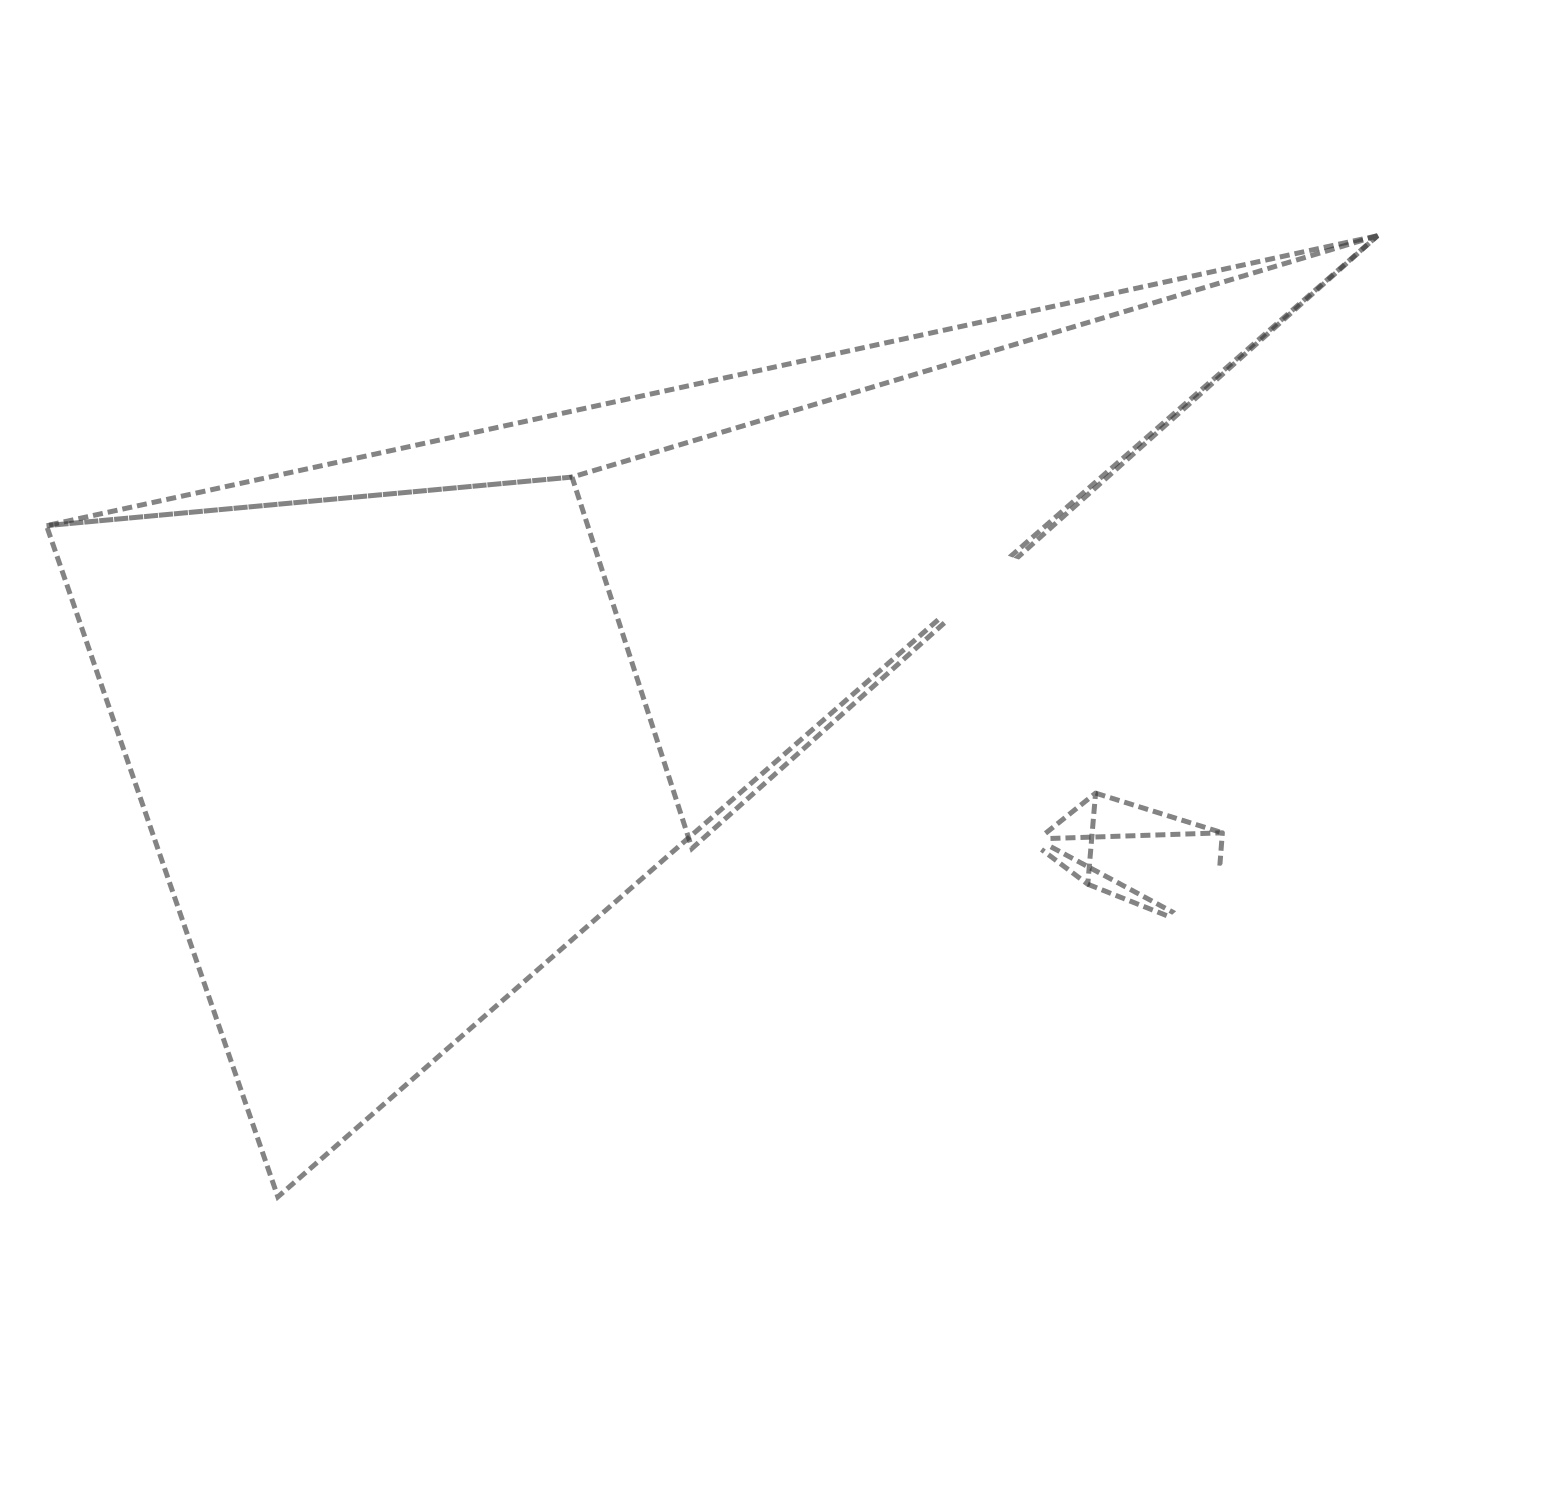
\includegraphics[width=\linewidth]{human-perspective-small}
             
        \end{column}
        \begin{column}{0.6\linewidth}
        
    \centering
    What about

    {\bf ``Give me \emph{that} book''}?

     \footnotesize
    (or even: {\bf ``Give me \emph{that}!''})

       \end{column}
    \end{columns}




\end{frame}
}

%\videoframe[0.56]{videos/this_box.webm}
\videoframe[0.56]{videos/this_box.mp4?autostart&start=1}

\begin{frame}{Example of first-order logic reasoning}
    \centering

    \vspace*{2em}
    ``Where is the other tape?''\\
    $\downarrow$\\
    find({\tt\scriptsize ?obj isAt ?loc, ?obj type VideoTape, ?obj differentFrom
    WALL\_E\_TAPE})

    \pause

    \vspace*{2em}
    Symbolic approaches effective at dealing with this kind of constraints

\end{frame}


%%%%%%%%%%%%%%%%%%%%%%%%%%%%%%%%%%%%%%%%%%%%%%%%%%%%%%%%%
%
\section[Theory of Mind]{One step further: Theory of Mind}
%
%%%%%%%%%%%%%%%%%%%%%%%%%%%%%%%%%%%%%%%%%%%%%%%%%%%%%%%%%
{ \paper{Wimmer and Perner, {\bf Beliefs about beliefs: Representation and
constraining function [...]}, Cognition, 1983]%\newline
%        [Lemaignan, Dillenbourg {\bf Mutual Modelling in Robotics: Inspirations
%        for the Next Steps} -- HRI 2015
}
\begin{frame}{1st order ToM: the False-Belief Experiment}

        \begin{center} 
            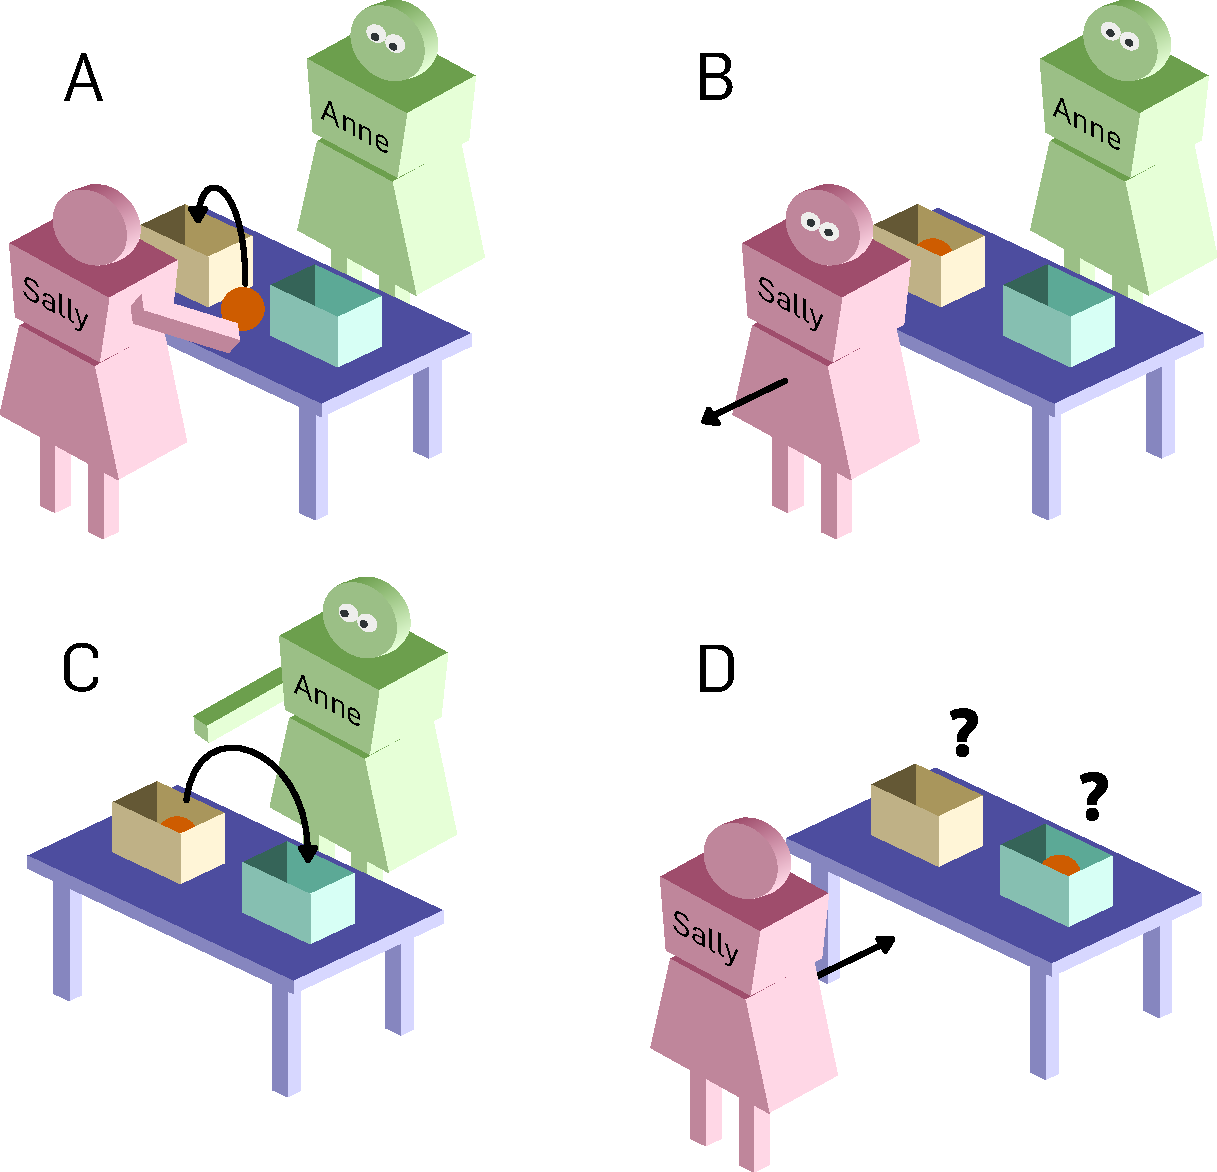
\includegraphics[width=0.7\textwidth]{sally_ann.pdf}
        \end{center}
\end{frame}
}

\begin{frame}[plain]

    \begin{center}
        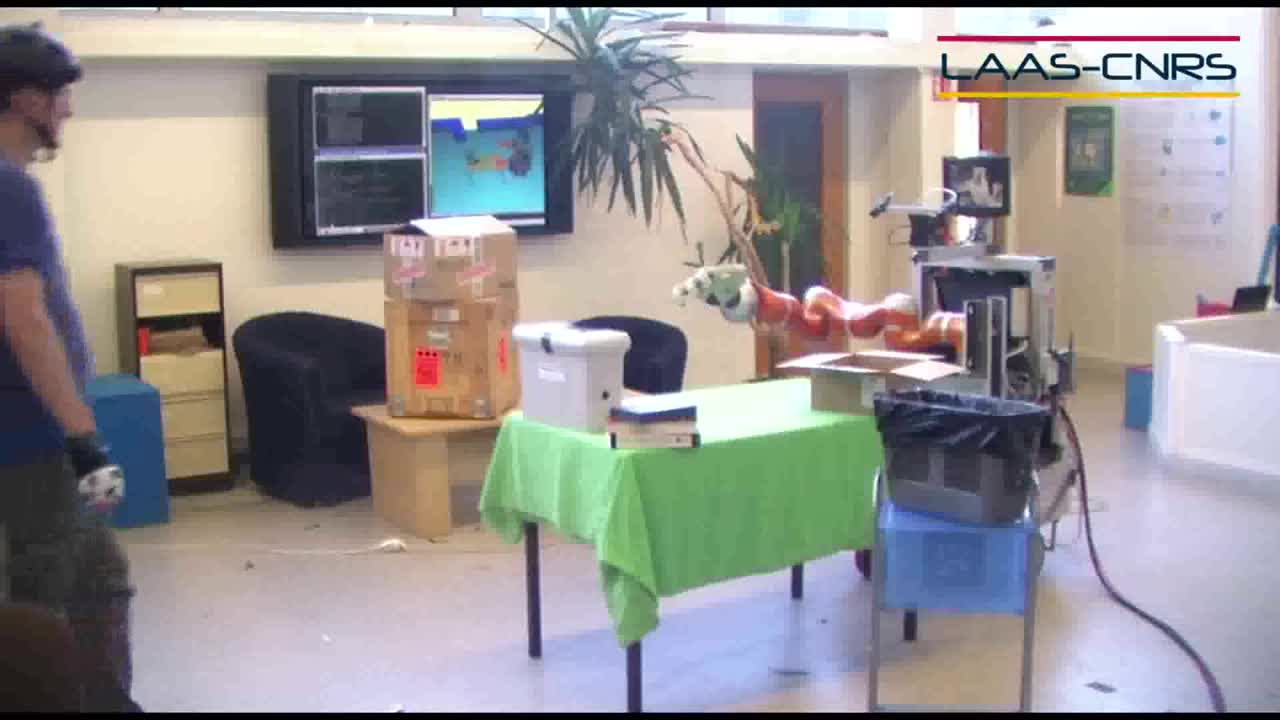
\includegraphics[width=0.8\linewidth]{videos/this_box_thumb}

        What if I ask for the video tape in the box, but the robot previously
        moved it somewhere else?


    \pause

        {\bf False-belief situation}
    \end{center}
\end{frame}

%%%%%%%%%%%%%%%%%%%%%%%%%%%%%%%%%%%%%%%%%%%%%%%%%%%%%%%%%

\begin{frame}{Parallel Models: towards theory of mind}
        \begin{multicols}{2}
            \begin{figure}
                \resizebox{0.4\textwidth}{!}{
                    \begin{tikzpicture}[
                        >=latex,
                        every edge/.style={<-, draw, very thick},
                        every node/.style={draw, font=\sf, node distance=0.5, rounded corners,
                                        align=center, inner sep=5pt,fill=hriSec2Dark!50},
                        classof/.style={<-, draw=black!60, dashed},
                        property/.style={<-, draw=hriSec2Comp},
                        propname/.style={above, draw=none, fill=none, font=\tt, inner sep=2pt},
                        instance/.style={draw=hriSec1Dark, font=\sf, node distance=0.5, rounded corners,
                        align=center, inner sep=5pt, fill=white}]

                    \node[fill=hriSec2Comp!50] (thing) {\textbf{thing}};
                    \node [fill=hriSec3CompDark!50, node distance=1.8, below left=of thing](sthing) {place} edge[dashed] (thing);
                    \node [fill=hriSec3CompDark!50, below left=of sthing] (agent) {agent} edge (sthing);
                        \node [fill=hriSec3CompDark!50, below=of sthing] (artifact) {artifact} edge (sthing);
                        \node [fill=hriSec3CompDark!50, below right=of sthing] (location) {physical
                        support} edge (sthing);
                        \node [fill=hriSec3CompDark!50, below right=of artifact] (table) {table}
                            edge (location) edge (artifact);


                    \node [node distance=1, below right=of thing] (tthing) {temporal thing} edge (thing);
                        \node [below right=of tthing] (evt) {event} edge[dashed] (tthing);
                                    \node [below right=of evt] (act) {action} edge (evt);

                \draw[dotted, thick] (-7,-5) -- (7.5, -5);

                \node [instance, below=3 of agent] (human) {human\_1} edge[classof, bend left] (agent);
                \node [instance, above left=of human] (human2) {human\_2} edge[classof, bend left] (agent);
                \node [instance, above right=of human, anchor=south] (robot) {pr2\_robot} edge[classof, bend left] (agent);
;
                \node [instance, right=of human, anchor=north west] (book) {harry\_potter}
                edge[classof] (artifact);
                \node [instance, right=3 of robot] (ikea) {ikea\_table} edge[classof, bend
                right] (table);
                \node [instance, right=2 of book] (red) {red} edge[property] node[propname] {hasColor} (book);

                \node [instance,right=1 of robot,fill=hriSec2] {myself} edge[property] node[propname, auto,above] {$\equiv$} (robot);

                \draw[dotted, thick] (-7,-8) -- (7.5, -8);

                \path (book.200) edge [property, out=-100, in=-80, looseness=2]
                node[propname,auto] {isNextTo} (human.south);
                \path (book.270) edge [property, out=-100, in=-90, looseness=3.5] node[propname,auto] {looksAt} (robot.south);
                \path (ikea.south) edge [property, out=-90, in=-80, looseness=3] node[propname, auto] {isOn} (book.320);
                \end{tikzpicture}
            }

            \end{figure}
            \begin{figure}
                \resizebox{0.4\textwidth}{!}{
                    \begin{tikzpicture}[
                        >=latex,
                        every edge/.style={<-, draw, very thick},
                        every node/.style={draw, font=\sf, node distance=0.5, rounded corners,
                                        align=center, inner sep=5pt,fill=hriSec2Dark!50},
                        classof/.style={<-, draw=black!60, dashed},
                        property/.style={<-, draw=hriSec2Comp},
                        propname/.style={above, draw=none, fill=none, font=\tt, inner sep=2pt},
                        instance/.style={draw=hriSec1Dark, font=\sf, node distance=0.5, rounded corners,
                        align=center, inner sep=5pt, fill=white}]

                    \node[fill=hriSec2Comp!50] (thing) {\textbf{thing}};
                    \node [fill=hriSec3CompDark!50, node distance=1.8, below left=of thing](sthing) {place} edge[dashed] (thing);
                    \node [fill=hriSec3CompDark!50, below left=of sthing] (agent) {agent} edge (sthing);
                        \node [fill=hriSec3CompDark!50, below=of sthing] (artifact) {artifact} edge (sthing);
                        \node [fill=hriSec3CompDark!50, below right=of sthing] (location) {physical
                        support} edge (sthing);
                        \node [fill=hriSec3CompDark!50, below right=of artifact] (table) {table}
                            edge (location) edge (artifact);


                    \node [node distance=1, below right=of thing] (tthing) {temporal thing} edge (thing);
                        \node [below right=of tthing] (evt) {event} edge[dashed] (tthing);
                                    \node [below right=of evt] (act) {action} edge (evt);

                \draw[dotted, thick] (-7,-5) -- (7.5, -5);

                \node [instance, below=3 of agent] (human) {human\_1} edge[classof, bend left] (agent);
                \node [instance, above left=of human] (human2) {human\_2} edge[classof, bend left] (agent);
                \node [instance, above right=of human, anchor=south] (robot) {pr2\_robot} edge[classof, bend left] (agent);
;
                \node [instance, right=of human, anchor=north west] (book) {harry\_potter}
                edge[classof] (artifact);
                \node [instance, right=3 of robot] (ikea) {ikea\_table} edge[classof, bend
                right] (table);
                \node [instance, right=2 of book] (red) {red} edge[property] node[propname] {hasColor} (book);

                \node [instance,below left=1 of human,fill=hriSec2] {myself} edge[property] node[propname, auto,above] {$\equiv$} (human);

                \draw[dotted, thick] (-7,-8) -- (7.5, -8);

                \path (book.200) edge [property, out=-100, in=-80, looseness=2]
                node[propname,auto] {isNextTo} (human.south);
                \path (book.270) edge [property, out=-100, in=-90, looseness=3.5] node[propname,auto] {looksAt} (robot.south);
                \path (ikea.south) edge [property, out=-90, in=-80, looseness=3] node[propname, auto] {isOn} (book.320);
                \end{tikzpicture}
            }
            \end{figure}
            \begin{figure}
                \resizebox{0.4\textwidth}{!}{
                    \begin{tikzpicture}[
                        >=latex,
                        every edge/.style={<-, draw, very thick},
                        every node/.style={draw, font=\sf, node distance=0.5, rounded corners,
                                        align=center, inner sep=5pt,fill=hriSec2Dark!50},
                        classof/.style={<-, draw=black!60, dashed},
                        property/.style={<-, draw=hriSec2Comp},
                        propname/.style={above, draw=none, fill=none, font=\tt, inner sep=2pt},
                        instance/.style={draw=hriSec1Dark, font=\sf, node distance=0.5, rounded corners,
                        align=center, inner sep=5pt, fill=white}]

                    \node[fill=hriSec2Comp!50] (thing) {\textbf{thing}};
                    \node [fill=hriSec3CompDark!50, node distance=1.8, below left=of thing](sthing) {place} edge[dashed] (thing);
                    \node [fill=hriSec3CompDark!50, below left=of sthing] (agent) {agent} edge (sthing);
                        \node [fill=hriSec3CompDark!50, below=of sthing] (artifact) {artifact} edge (sthing);
                        \node [fill=hriSec3CompDark!50, below right=of sthing] (location) {physical
                        support} edge (sthing);
                        \node [fill=hriSec3CompDark!50, below right=of artifact] (table) {table}
                            edge (location) edge (artifact);


                    \node [node distance=1, below right=of thing] (tthing) {temporal thing} edge (thing);
                        \node [below right=of tthing] (evt) {event} edge[dashed] (tthing);
                                    \node [below right=of evt] (act) {action} edge (evt);

                \draw[dotted, thick] (-7,-5) -- (7.5, -5);

                \node [instance, below=3 of agent] (human) {human\_1} edge[classof, bend left] (agent);
                \node [instance, above left=of human] (human2) {human\_2} edge[classof, bend left] (agent);
                \node [instance, above right=of human, anchor=south] (robot) {pr2\_robot} edge[classof, bend left] (agent);
;
                \node [instance, right=of human, anchor=north west] (book)
                        {harry\_potter}
                edge[classof] (artifact);
                \node [instance, right=3 of robot] (ikea) {ikea\_table} edge[classof, bend
                right] (table);
                \node [instance, right=2 of book] (red) {red} edge[property] node[propname] {hasColor} (book);

                \node [instance,below=1 of human2,fill=hriSec2] {myself} edge[property] node[propname, auto] {$\equiv$} (human2);

                \draw[dotted, thick] (-7,-8) -- (7.5, -8);

                \path (book.200) edge [property, out=-100, in=-80, looseness=2]
                node[propname,auto] {isNextTo} (human.south);
                \path (book.270) edge [property, out=-100, in=-90, looseness=3.5] node[propname,auto] {looksAt} (robot.south);
                \path (ikea.south) edge [property, out=-90, in=-80, looseness=3] node[propname, auto] {isOn} (book.320);
                \end{tikzpicture}
            }
            \end{figure}
            {\vspace*{1.5cm}\hspace*{2.5cm}\huge...}
        \end{multicols}

\end{frame}

%%%%%%%%%%%%%%%%%%%%%%%%%%%%%%%%%%%%%%%%%%%%%%%%%%%%%%%%%%%%%%%%%
%%%%%%%%%%%%%%%%%%%%%%%%%%%%%%%%%%%%%%%%%%%%%%%%%%%%%%%%%%%%%%%%%
%%%%%%%%%%%%%%%%%%%%%%%%%%%%%%%%%%%%%%%%%%%%%%%%%%%%%%%%%%%%%%%%%

\section{Semantics-aware architecture}

{
    \paper{Lemaignan et al., {\bf Artificial Cognition for Social Human-Robot
    Interaction: An Implementation}, Artifical Intelligence, 2017}
\begin{frame}<1-6>{Into an control architecture}
    \begin{figure}
        \centering

        \resizebox{0.9\paperwidth}{!}{%

            
            \newcommand{\dimming}{50}

            \tikzset{subpart/.style={draw, font=\scriptsize, fill opacity=0.5, text opacity=1, fill=white!50}}

            \begin{tikzpicture}[
                    >=latex,
                    every edge/.style={draw, very thick},
                    skill/.style={draw, rounded corners, align=center, inner sep=5pt, fill=black!20},
                label/.style={midway, align=center, font=\scriptsize, fill=white}]

                %%% Separation between deliberative layer and sensori-motor layer
                \draw[dotted, thick] (-8,-5) -- (12, -5);

                %%% SPARK
                \uncover<2->{
                    \node at (4,-3.5)[skill, fill=hriSec3!\dimming] (spark) {%
                    \begin{tikzpicture}
                        \node at (0,0) (geom) {Geometric \& Temporal Reasoning};
                        \node [subpart, below=0.2 of geom.south west, anchor=north west] (world-update) {Sensors fusion};
                        \node [subpart, right=0.2 of world-update] (geom-model) {Geometric model of the environment};
                        \node [subpart, right=0.2 of geom-model] (fact-prod) {Symbolic facts production};
                    \end{tikzpicture}
                };
                }

                %%% LOWLEVEL
                \node [skill, below=0.7 of spark,fill=gray!\dimming] (lowlevel) {%
                    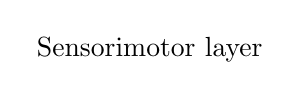
\begin{tikzpicture}
                        \node at (0,0) (sensori) {Sensorimotor layer};
                        %\node [subpart, below=0.2 of sensori.south west, anchor=north west, align=left] (perception) {{\bf Perception} \\ 2D markers, RGB-D, motion capture};
                        %\node [subpart, align=right, right=0.2 of perception] {{\bf Actuation} \\ Head's pan-tilt unit, grippers, arms, wheels};
                    \end{tikzpicture}
                };

                \uncover<2->{
                \path (lowlevel) edge [->] (spark);
                }

                %%% ORO
                \uncover<3->{
                \node at (0,0)[skill, ultra thick, fill=hriSec2Dark!50] (oro)
                {Symbolic facts \\ and beliefs management};
                \path (spark.100) edge [->, bend right] node[label] {symbolic \\ facts} (oro);
                }

                %%% HATP
                \uncover<5->{
                \node at (-6, 2.5)[skill, fill=hriSec1!\dimming] (hatp) {Human-aware
                symbolic \\task planning};
                \path (hatp) edge [<->, bend right] node[label] {world model and \\ agents beliefs} (oro.170);
                }

                %%% DIALOGS
                \uncover<4->{
                \node at (-6, -3) [skill, fill=hriSec3Dark!50] (dialogs)
                {Dialogue processing};
                \path (dialogs) edge [<->, bend left] node[label] {natural language \\ grounding} (oro.190);
                }
                %%% SHARY
                \uncover<5->{
                \node at (4,4.5)[skill, fill=hriSec1Comp!\dimming] (shary) {%
                    \begin{tikzpicture}
                        \node at (0,0) (exec) {Execution Controller};
                        \node [subpart, below=0.2 of exec.south west, anchor=north west] (plans) {Goal \& Plans \\ management};
                        \node [subpart, right=0.2 of plans] (sit-asses) {Situation assessment \\ and context management};
                        \node [subpart, right=0.2 of sit-asses] {Action instantiation, \\ execution and monitoring};
                    \end{tikzpicture}
                };
                \path (shary) edge [<->, bend left] node[label] {events, \\ world model and \\ agents beliefs} (oro);
                \path (shary) edge [<->, bend left, looseness=0.8] node[label] {action monitoring \\ and management of \\ position hypotheses} (spark);
                \path (shary.west) edge [<->, bend right] node[label] {shared \\ plans} (hatp);
                }
                %%% MHP
                \uncover<6->{
                \node at (9,0)[skill, fill=hriSec3CompDark!\dimming] (mhp)
                {Human-aware Motion \\ and Manipulation Planning};
                \path (shary.340) edge [<->, bend left] node[label] {motion plan \\ requests} (mhp);
                \path (spark.5) edge [->, bend right] node[label] {environment\\model} (mhp);
                \path (lowlevel.east) edge [<-, bend right=60, looseness=1.3] node[label] {atomic\\actions} (mhp.south east);
                }



            \end{tikzpicture}
        }
    \end{figure}


\end{frame}
%}


\videoframe[0.7]{videos/clean-table.webm}

%%%%%%%%%%%%%%%%%%%%%%%%%%%%%%%%%%%%%%%%%%%%%%%%%%%%%%%%
%{
%\paper{Lemaignan et al. {\bf Artificial Cognition for Social Human-Robot
%     Interaction: An Implementation} Artifical Intelligence, 2016}
\begin{frame}{Full social \& autonomous interaction: one example}

    \begin{center}

     \begin{columns}
         \begin{column}{0.3\linewidth}
                 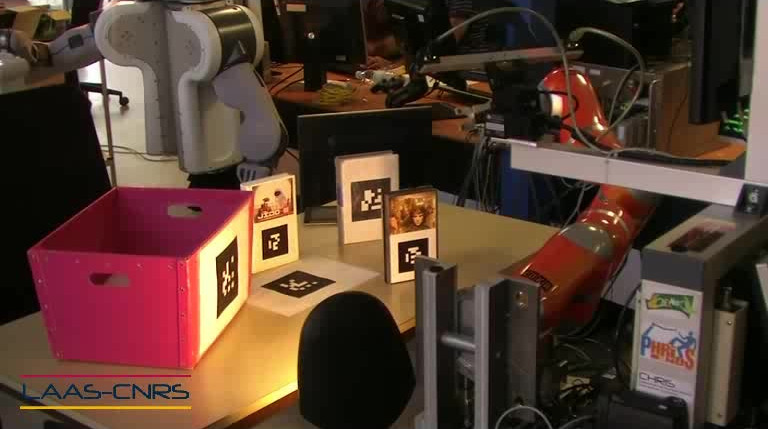
\includegraphics[height=0.75\paperheight]{clean-table}
         \end{column}
         \begin{column}{0.7\linewidth}
             \centering
             \resizebox{!}{0.75\paperheight}{%
                 \begin{tikzpicture}[
                         >=latex,
                     every edge/.style={draw, ultra thick, ->},
                     every node/.style={align=center},
                     robot/.style={fill=hriSec2Comp!50},
                     plan/.style={draw,
                      thick,  
                      circle, 
                      font=\sf,
                      align=center,
                      fill=hriSec3CompDark!50, 
                      minimum size=1cm, 
                      inner sep=0.1cm}
                  ]

                     \coordinate (figbottom) at (-0.5, -28.5);


                     \fill[gray!10!white] (4.6,.5) rectangle (figbottom);

                     \path (-0.5,0) edge (figbottom) node[sloped, above left, rotate=90] {\large\bf time};

                     \node at (2,0) (percept) {\bf Perception};
                     \node[below=0.5 of percept.south west, anchor=mid] {camera};
                     \node[below=0.5 of percept.south east, anchor=mid] {3D model};

                     \node[right=4 of percept, minimum width=2.5cm] (kb) {\bf Knowledge};
                     \node[below=0.5 of kb.south west, anchor=mid east] (kbr) {robot};
                     \node[below=0.5 of kb.south east, anchor=mid west] (kbh) {human};
                     \draw[dotted] (kbr) to (figbottom -| kbr);
                     \draw[dotted] (kbh) to (figbottom -| kbh);

                     \fill[gray!10!white] (12,.5) rectangle (17,0 |- figbottom);
                     \node[right=4.5 of kb] (plan) {\bf Plan};
                     \node[below=0.5 of plan.south west, anchor=mid east] (probot) {robot};
                     \node[below=0.5 of plan.south east, anchor=mid west] (phuman) {human};
                     \draw[dotted] (probot) to (figbottom -| probot);
                     \draw[dotted] (phuman) to (figbottom -| phuman);

                     \node[right=5 of plan] (action) {\bf Actions};
                     \node[below=0.5 of action.south west, anchor=mid east] (arobot) {robot};
                     \node[below=0.5 of action.south east, anchor=west] (ahuman) {human\\(monitoring)};
                     \draw[dotted] (arobot) to (figbottom -| arobot);
                     \draw[dotted] (ahuman) to (figbottom -| ahuman);

                     \draw[dashed] (-0.6,-1.2) --(24, -1.2);

                     \node[anchor=east] at (-0.5, -3) (t1) {\Large $t_1$};
                     \node[anchor=east, below=6 of t1] (t2) {\Large $t_2$};
                     \node[anchor=east, below=6 of t2] (t3) {\Large $t_3$};
                     \node[anchor=east, below=4 of t3] (t4) {\Large $t_4$};
                     \node[anchor=east, below=5 of t4] (t5) {\Large $t_5$};

                     %%%%%%%%%%%%%%%%%%%%%%%%%%%%%%%%%%%%%%%%%%%%%%%%%%%%%%%%%%%%%%%%%%%%%%%%%%%%%%%%%%%%%%%%%%%%
                     %%% PERCEPTIONS
                     %%%%%%%%%%%%%%%%%%%%%%%%%%%%%%%%%%%%%%%%%%%%%%%%%%%%%%%%%%%%%%%%%%%%%%%%%%%%%%%%%%%%%%%%%%%%

         \node at (t1 -| percept) (cam1) {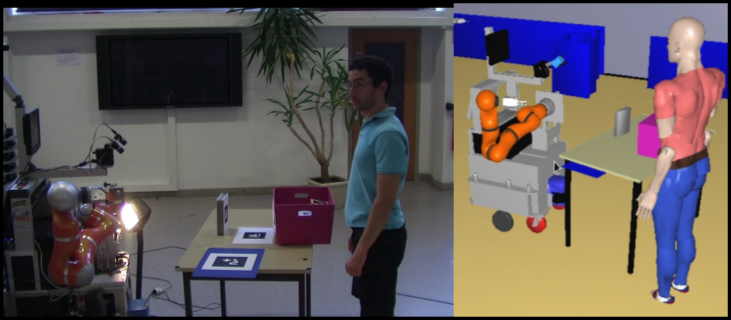
\includegraphics[height=2cm]{cleantable/manip_run_cam1.png}};
         \node at (t2 -| percept) (cam2) {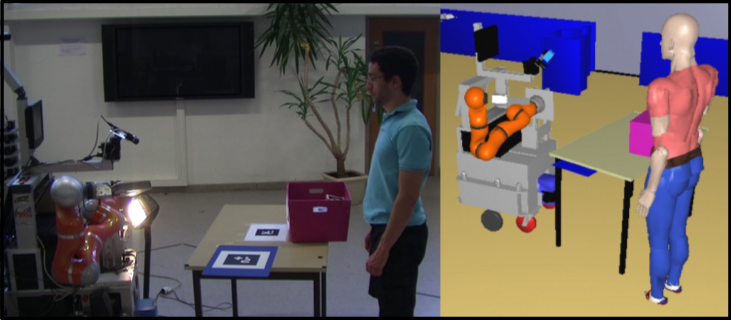
\includegraphics[height=2cm]{cleantable/manip_run_cam2.png}};
         \node at (t3 -| percept) (cam3) {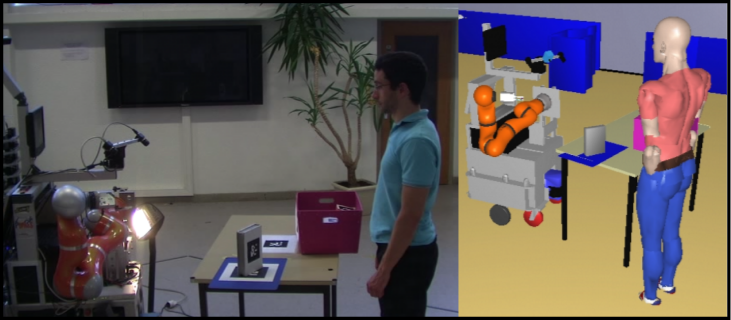
\includegraphics[height=2cm]{cleantable/manip_run_cam3.png}};
         \node at (t4 -| percept) (cam4) {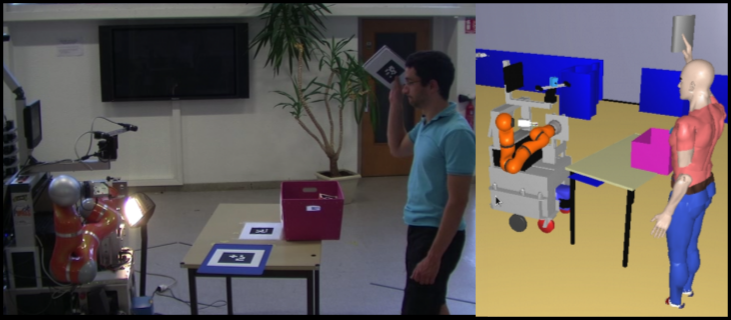
\includegraphics[height=2cm]{cleantable/manip_run_cam4.png}};
         \node at (t5 -| percept) (cam5) {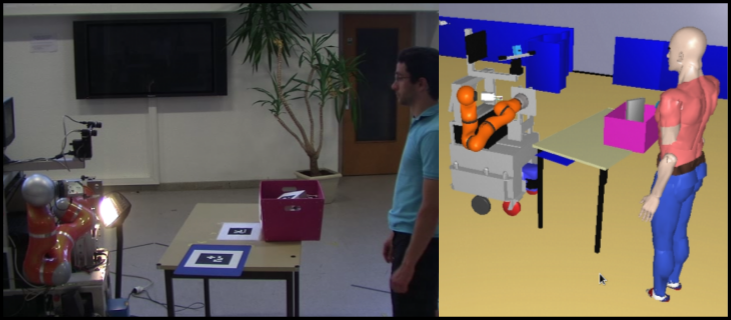
\includegraphics[height=2cm]{cleantable/manip_run_cam5.png}};

         %%%%%%%%%%%%%%%%%%%%%%%%%%%%%%%%%%%%%%%%%%%%%%%%%%%%%%%%%%%%%%%%%%%%%%%%%%%%%%%%%%%%%%%%%%%%
         %%% KNOWLEDGE
         %%%%%%%%%%%%%%%%%%%%%%%%%%%%%%%%%%%%%%%%%%%%%%%%%%%%%%%%%%%%%%%%%%%%%%%%%%%%%%%%%%%%%%%%%%%%

         \node[fill=white,align=left] at (cam1 -| kbr) (kb1) {\stmt{TAPE isVisible true}\\
                                                    \stmt{TAPE isReachable true}\\
                                                    \stmt{TAPE isOn TABLE}\\
                                                    \stmt{BIN isVisible true}\\
                                                    \stmt{BIN isReachable false}};

         \node[fill=white,align=left] at (cam1 -| kbh) {\stmt{TAPE isVisible true}\\
                                                    \stmt{TAPE isReachable false}\\
                                                    \stmt{TAPE isOn TABLE}\\
                                                    \stmt{BIN isVisible true}\\
                                                    \stmt{BIN isReachable true}};

         \node[fill=white,align=left] at (cam2 -| kbr) (kb2) {\stmt{ROBOT hasInHand TAPE}};


         \node[fill=white,align=left] at (cam3 -| kbr) {\stmt{TAPE isReachable true}\\
                                        \stmt{TAPE isVisible true} \\
                                        \stmt{TAPE isOn TABLE}};

         \node[fill=white,align=left ] at (cam3 -| kbh) (kb3) {\stmt{TAPE isReachable true}\\
                                         \stmt{TAPE isVisible true}};

         \node[fill=white,align=left] at (cam4 -| kbh) (kb4) {\stmt{HUMAN hasInHand TAPE}};

         \node[fill=white,align=left] at (cam5 -| kbr)  {\stmt{TAPE isIn BIN}};
         \node[fill=white,align=left] at (cam5 -| kbh) (kb5) {\stmt{TAPE isIn BIN}};

         %%%%%%%%%%%%%%%% %%%%%%%%%%%%%%%%%%%%%%%%%%%%%%%%%%%%%%%%%%%%%%%%%%%%%%%%%%%%%%%%%%%%%%%%%%%%
         %%% PLANS
         %%%%%%%%%%%%%%%%%%%%%%%%%%%%%%%%%%%%%%%%%%%%%%%%%%%%%%%%%%%%%%%%%%%%%%%%%%%%%%%%%%%%%%%%%%%%

         \node[fill=gray!10!white,below=1 of plan] (incoming) {\bf \Large Incoming goal \\ \it Clean the table!};

         \node[anchor=north, plan, robot] at (cam1.south -| probot) (pr1) {\bf TAKE\\TAPE\\TABLE};
         \node[anchor=north, plan, robot] at (cam2.south -| probot)  (pr2) {\bf PUTRV\\TAPE\\TABLE} edge[<-] (pr1);
         \node[anchor=north, plan] at (cam3.south -| phuman) (ph1) {\bf TAKE\\TAPE\\TABLE} edge[<-] (pr2);
         \node[anchor=north, plan]  at (cam4.south -| phuman) (ph2) {\bf PUT\\TAPE\\BIN} edge[<-] (ph1);

         \node[fill=gray!10!white,anchor=north] at (cam5.south -| plan) (done) {\bf \Large Goal completed};

         %%%%%%%%%%%%%%%%%%%%%%%%%%%%%%%%%%%%%%%%%%%%%%%%%%%%%%%%%%%%%%%%%%%%%%%%%%%%%%%%%%%%%%%%%%%%
         %%% ACTIONS
         %%%%%%%%%%%%%%%%%%%%%%%%%%%%%%%%%%%%%%%%%%%%%%%%%%%%%%%%%%%%%%%%%%%%%%%%%%%%%%%%%%%%%%%%%%%%

         \only{
             \node[fill=white] at (pr1 -| arobot) (ep1) {\it evaluate pre-conditions};

         \node[below=0.1 of ep1] (mhp1) {%
             \begin{tikzpicture}
                 \node[fill=white] (title) {\bf motion planning};
                 \node[below=0.1 of title.south west, label=below:{\tt PICK\_GOTO}] (mapg) {
\includegraphics{cleantable/MHP_ARM_PICK_GOTO}};
                 \node[fill=white,right=of mapg, label=below:{\tt TAKE\_TO\_FREE}] (mattf) {
\includegraphics{cleantable/MHP_ARM_TAKE_TO_FREE}} edge[<-] (mapg);
             \end{tikzpicture}
         };
         \node[fill=white,below=0.1 of mhp1] (me1) {\bf motion execution};
         \node[fill=white,below=0.1 of me1] (ae1) {\it assess post-conditions};
     }
     %%%%%%%%%%%%%%%%%%%%%%%%%%%%%%%%%%%%%%%%%%%%%%%%%%%%%%%%%%%%%%%%%%%%%%%%%%%%%%%%%%%%%%%%%%%%%
         \only{
             \node[fill=white] at (pr2 -| arobot) (ep2) {\it evaluate pre-conditions};

         \node[below=0.1 of ep2] (mhp2) {%
             \begin{tikzpicture}
                 \node[fill=white] (title) {\bf motion planning};
                 \node[fill=white,below=0.1 of title, label=below:{\tt ESCAPE}] (maeo) {
\includegraphics{cleantable/MHP_ARM_ESCAPE_OBJECT}};
                 \node[left=of maeo, label=below:{\tt PLACE\_FROM\_FREE}] (mapff) {
\includegraphics{cleantable/MHP_ARM_PLACE_FROM_FREE}} edge (maeo);
                 \node[fill=white,right=of maeo, label=below:{\tt TO\_FREE}] (maf) {
\includegraphics{cleantable/MHP_ARM_FREE}} edge[<-] (maeo);
             \end{tikzpicture}
         };
         \node[fill=white,below=0.1 of mhp2] (me2) {\bf motion execution};
         \node[fill=white,below=0.1 of me2] (ae2) {\it assess post-conditions};
     }
     %%%%%%%%%%%%%%%%%%%%%%%%%%%%%%%%%%%%%%%%%%%%%%%%%%%%%%%%%%%%%%%%%%%%%%%%%%%%%%%%%%%%%%%%%%%%%

         \node[anchor=north] at (ph1 -| ahuman) (wait1) {%
             \begin{tikzpicture}
                 \node[fill=white] (title) {\it wait for pick\\ {\tt TAPE} \it from {\tt TABLE}};
                 \node[below=0.1 of title] {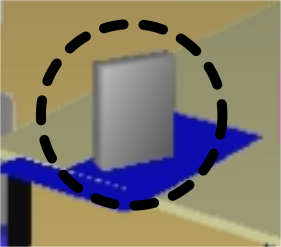
\includegraphics{cleantable/wait_for_pick}};
             \end{tikzpicture}
         };

         \node[anchor=north] at (ph2 -| ahuman) (wait2) {%
             \begin{tikzpicture}
                 \node[fill=white] (title) {\it wait for put\\ {\tt TAPE} \it into {\tt BIN}};
                 \node[below=0.1 of title] {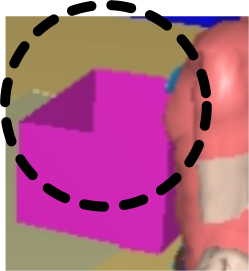
\includegraphics{cleantable/wait_for_throw}};
             \end{tikzpicture}
         };


         %%%%%%%%%%%%%%%%%%%%%%%%%%%%%%%%%%%%%%%%%%%%%%%%%%%%%%%%%%%%%%%%%%%%%%%%%%%%%%%%%%%%%%%%%%%%
         %%% FLOW
         %%%%%%%%%%%%%%%%%%%%%%%%%%%%%%%%%%%%%%%%%%%%%%%%%%%%%%%%%%%%%%%%%%%%%%%%%%%%%%%%%%%%%%%%%%%%
         \draw[dotted, ->, in=45, out=180] (incoming.west) to (kb1);
         \draw[dotted, ->, bend right] (kb1) to (pr1);
         \draw[dotted, ->, bend left] (pr1) to (ep1);
         \draw[dotted, ->, in=45, out=180] (ae1.west) to (kb2);
         \draw[dotted, ->, bend right] (kb2) to (pr2);
         \draw[dotted, ->, bend left] (pr2) to (ep2);
         \draw[dotted, ->, in=45, out=180] (ae2.west) to (kb3);
         \draw[dotted, ->, bend right] (kb3) to (ph1);
         \draw[dotted, ->, bend left] (ph1) to (wait1);
         \draw[dotted, ->, in=-20, out=180] (wait1.west) to (kb4.east);
         \draw[dotted, ->, bend right] (kb4) to (ph2);
         \draw[dotted, ->, bend left] (ph2) to (wait2);
         \draw[dotted, ->, in=20, out=180] (wait2.west) to (kb5);
         \draw[dotted, ->, bend left] (kb5.east) to (done.north);


     \end{tikzpicture}
      }
         \end{column}
     \end{columns}
    \end{center}

\end{frame}
}

\begin{frame}{``Cleaning the table''...}
\centering

\resizebox{!}{0.75\paperheight}{%
\begin{tikzpicture}[
        >=latex,
        every edge/.style={draw, ultra thick, ->},
        every node/.style={align=center},
        robot/.style={fill=hriSec2Comp!50},
        plan/.style={draw,
                     thick,  
                     circle, 
                     font=\sf,
                     align=center,
                     fill=hriSec3CompDark!50, 
                     minimum size=1cm, 
                     inner sep=0.1cm}
        ]

        \coordinate<1> (figbottom) at (-0.5, -28.5);
        \coordinate<2-5> (figbottom) at (-0.5, -10.5);
        \node<2-5> at (0,5) {};
        \node<2-5> at ($(figbottom) + (0,-5)$) {};


        \fill[gray!10!white] (4.6,.5) rectangle (figbottom);

        \path (-0.5,0) edge (figbottom) node[sloped, above left, rotate=90] {\large\bf time};

        \node at (2,0) (percept) {\bf Perception};
            \node[below=0.5 of percept.south west, anchor=mid] {camera};
            \node[below=0.5 of percept.south east, anchor=mid] {3D model};

        \node[right=4 of percept, minimum width=2.5cm] (kb) {\bf Knowledge};
            \node[below=0.5 of kb.south west, anchor=mid east] (kbr) {robot};
            \node[below=0.5 of kb.south east, anchor=mid west] (kbh) {human};
            \draw[dotted] (kbr) to (figbottom -| kbr);
            \draw[dotted] (kbh) to (figbottom -| kbh);

        \fill[gray!10!white] (12,.5) rectangle (17,0 |- figbottom);
        \node[right=4.5 of kb] (plan) {\bf Plan};
            \node[below=0.5 of plan.south west, anchor=mid east] (probot) {robot};
            \node[below=0.5 of plan.south east, anchor=mid west] (phuman) {human};
            \draw[dotted] (probot) to (figbottom -| probot);
            \draw[dotted] (phuman) to (figbottom -| phuman);

        \node[right=5 of plan] (action) {\bf Actions};
            \node[below=0.5 of action.south west, anchor=mid east] (arobot) {robot};
            \node[below=0.5 of action.south east, anchor=west] (ahuman) {human\\(monitoring)};
            \draw[dotted] (arobot) to (figbottom -| arobot);
            \draw[dotted] (ahuman) to (figbottom -| ahuman);

        \draw[dashed] (-0.6,-1.2) --(24, -1.2);

        \node<1,2>[anchor=east] at (-0.5, -3) (t1) {\Large $t_1$};
        \node<1,2>[anchor=east, below=6 of t1] (t2) {\Large $t_2$};
        \node<3>[anchor=east] at (-0.5, -3) (t2) {\Large $t_2$};
        \node<1,3>[anchor=east, below=6 of t2] (t3) {\Large $t_3$};
        \node<4>[anchor=east] at (-0.5, -3) (t3) {\Large $t_3$};
        \node<1,4>[anchor=east, below=4 of t3] (t4) {\Large $t_4$};
        \node<5>[anchor=east] at (-0.5, -3) (t4) {\Large $t_4$};
        \node<1,5>[anchor=east, below=5 of t4] (t5) {\Large $t_5$};

        %%%%%%%%%%%%%%%%%%%%%%%%%%%%%%%%%%%%%%%%%%%%%%%%%%%%%%%%%%%%%%%%%%%%%%%%%%%%%%%%%%%%%%%%%%%%
        %%% PERCEPTIONS
        %%%%%%%%%%%%%%%%%%%%%%%%%%%%%%%%%%%%%%%%%%%%%%%%%%%%%%%%%%%%%%%%%%%%%%%%%%%%%%%%%%%%%%%%%%%%

        \node<1,2> at (t1 -| percept) (cam1) {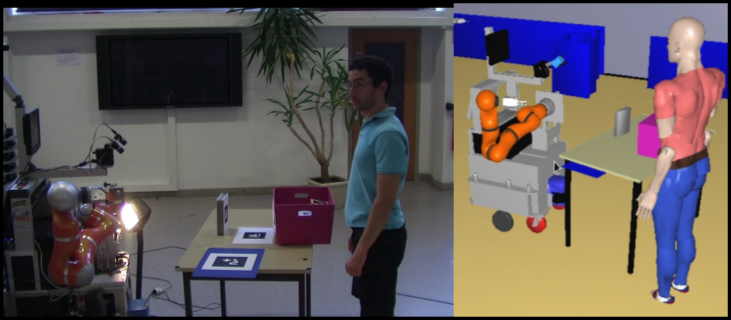
\includegraphics[height=2cm]{cleantable/manip_run_cam1.png}};
        \node<1,3> at (t2 -| percept) (cam2) {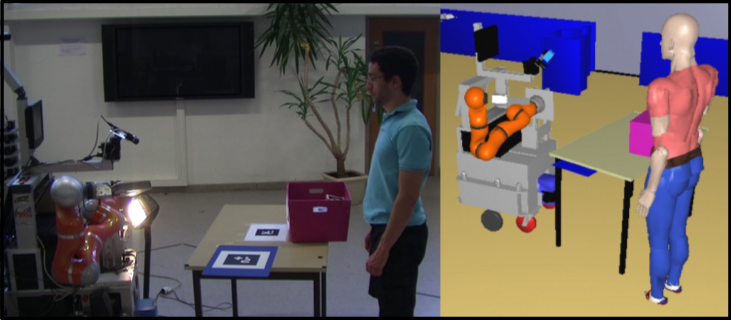
\includegraphics[height=2cm]{cleantable/manip_run_cam2.png}};
        \node<1,4> at (t3 -| percept) (cam3) {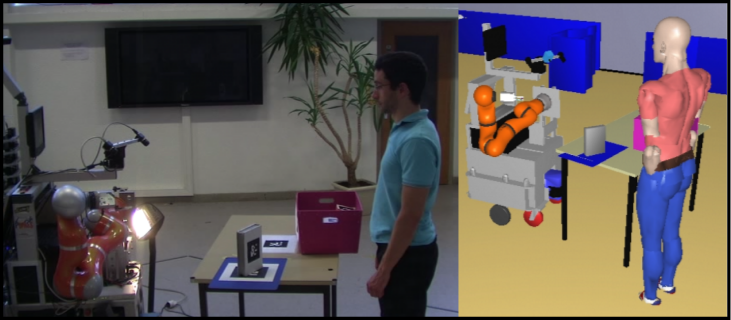
\includegraphics[height=2cm]{cleantable/manip_run_cam3.png}};
        \node<1,5> at (t4 -| percept) (cam4) {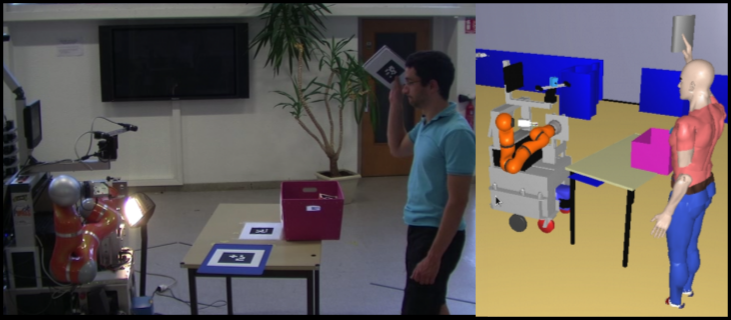
\includegraphics[height=2cm]{cleantable/manip_run_cam4.png}};
        \node<1,5> at (t5 -| percept) (cam5) {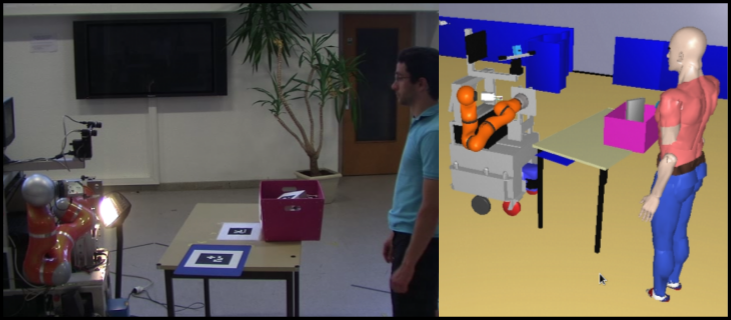
\includegraphics[height=2cm]{cleantable/manip_run_cam5.png}};

        %%%%%%%%%%%%%%%%%%%%%%%%%%%%%%%%%%%%%%%%%%%%%%%%%%%%%%%%%%%%%%%%%%%%%%%%%%%%%%%%%%%%%%%%%%%%
        %%% KNOWLEDGE
        %%%%%%%%%%%%%%%%%%%%%%%%%%%%%%%%%%%%%%%%%%%%%%%%%%%%%%%%%%%%%%%%%%%%%%%%%%%%%%%%%%%%%%%%%%%%

        \node<1,2>[fill=white,align=left] at (cam1 -| kbr) (kb1) {\stmt{TAPE isVisible true}\\
                                                        \stmt{TAPE isReachable true}\\
                                                        \stmt{TAPE isOn TABLE}\\
                                                        \stmt{BIN isVisible true}\\
                                                        \stmt{BIN isReachable false}};

        \node<1,2>[fill=white,align=left] at (cam1 -| kbh) {\stmt{TAPE isVisible true}\\
                                                        \stmt{TAPE isReachable false}\\
                                                        \stmt{TAPE isOn TABLE}\\
                                                        \stmt{BIN isVisible true}\\
                                                        \stmt{BIN isReachable true}};

        \node<1,3>[fill=white,align=left] at (cam2 -| kbr) (kb2) {\stmt{ROBOT hasInHand TAPE}};


        \node<1,4>[fill=white,align=left] at (cam3 -| kbr) {\stmt{TAPE isReachable true}\\
                                            \stmt{TAPE isVisible true} \\
                                            \stmt{TAPE isOn TABLE}};

        \node<1,4>[fill=white,align=left ] at (cam3 -| kbh) (kb3) {\stmt{TAPE isReachable true}\\
                                             \stmt{TAPE isVisible true}};

        \node<1,5>[fill=white,align=left] at (cam4 -| kbh) (kb4) {\stmt{HUMAN hasInHand TAPE}};

        \node<1,5>[fill=white,align=left] at (cam5 -| kbr)  {\stmt{TAPE isIn BIN}};
        \node<1,5>[fill=white,align=left] at (cam5 -| kbh) (kb5) {\stmt{TAPE isIn BIN}};

        %%%%%%%%%%%%%%%% %%%%%%%%%%%%%%%%%%%%%%%%%%%%%%%%%%%%%%%%%%%%%%%%%%%%%%%%%%%%%%%%%%%%%%%%%%%%
        %%% PLANS
        %%%%%%%%%%%%%%%%%%%%%%%%%%%%%%%%%%%%%%%%%%%%%%%%%%%%%%%%%%%%%%%%%%%%%%%%%%%%%%%%%%%%%%%%%%%%

        \node<1,2>[fill=gray!10!white,below=1 of plan] (incoming) {\bf \Large Incoming goal \\ \it Clean the table!};

        \node<1,2>[anchor=north, plan, robot] at (cam1.south -| probot) (pr1) {\bf TAKE\\TAPE\\TABLE};
        \node<1,3>[anchor=north, plan, robot] at (cam2.south -| probot)  (pr2) {\bf PUTRV\\TAPE\\TABLE} edge[<-] (pr1);
        \node<1,4>[anchor=north, plan] at (cam3.south -| phuman) (ph1) {\bf TAKE\\TAPE\\TABLE} edge[<-] (pr2);
        \node<1,5>[anchor=north, plan]  at (cam4.south -| phuman) (ph2) {\bf PUT\\TAPE\\BIN} edge[<-] (ph1);

        \node<1,5>[fill=gray!10!white,anchor=north] at (cam5.south -| plan) (done) {\bf \Large Goal completed};

        %%%%%%%%%%%%%%%%%%%%%%%%%%%%%%%%%%%%%%%%%%%%%%%%%%%%%%%%%%%%%%%%%%%%%%%%%%%%%%%%%%%%%%%%%%%%
        %%% ACTIONS
        %%%%%%%%%%%%%%%%%%%%%%%%%%%%%%%%%%%%%%%%%%%%%%%%%%%%%%%%%%%%%%%%%%%%%%%%%%%%%%%%%%%%%%%%%%%%

        \only<1,2>{
        \node[fill=white] at (pr1 -| arobot) (ep1) {\it evaluate pre-conditions};

        \node[below=0.1 of ep1] (mhp1) {%
            \begin{tikzpicture}
                \node[fill=white] (title) {\bf motion planning};
                \node[below=0.1 of title.south west, label=below:{\tt PICK\_GOTO}] (mapg) {
\includegraphics{cleantable/MHP_ARM_PICK_GOTO}};
                \node[fill=white,right=of mapg, label=below:{\tt TAKE\_TO\_FREE}] (mattf) {
\includegraphics{cleantable/MHP_ARM_TAKE_TO_FREE}} edge[<-] (mapg);
            \end{tikzpicture}
        };
        \node[fill=white,below=0.1 of mhp1] (me1) {\bf motion execution};
        \node[fill=white,below=0.1 of me1] (ae1) {\it assess post-conditions};
        }
        %%%%%%%%%%%%%%%%%%%%%%%%%%%%%%%%%%%%%%%%%%%%%%%%%%%%%%%%%%%%%%%%%%%%%%%%%%%%%%%%%%%%%%%%%%%%%
        \only<1,3>{
        \node[fill=white] at (pr2 -| arobot) (ep2) {\it evaluate pre-conditions};

        \node[below=0.1 of ep2] (mhp2) {%
            \begin{tikzpicture}
                \node[fill=white] (title) {\bf motion planning};
                \node[fill=white,below=0.1 of title, label=below:{\tt ESCAPE}] (maeo) {
\includegraphics{cleantable/MHP_ARM_ESCAPE_OBJECT}};
                \node[left=of maeo, label=below:{\tt PLACE\_FROM\_FREE}] (mapff) {
\includegraphics{cleantable/MHP_ARM_PLACE_FROM_FREE}} edge (maeo);
                \node[fill=white,right=of maeo, label=below:{\tt TO\_FREE}] (maf) {
\includegraphics{cleantable/MHP_ARM_FREE}} edge[<-] (maeo);
            \end{tikzpicture}
        };
        \node[fill=white,below=0.1 of mhp2] (me2) {\bf motion execution};
        \node[fill=white,below=0.1 of me2] (ae2) {\it assess post-conditions};
        }
        %%%%%%%%%%%%%%%%%%%%%%%%%%%%%%%%%%%%%%%%%%%%%%%%%%%%%%%%%%%%%%%%%%%%%%%%%%%%%%%%%%%%%%%%%%%%%

        \node<1,4>[anchor=north] at (ph1 -| ahuman) (wait1) {%
            \begin{tikzpicture}
                \node[fill=white] (title) {\it wait for pick\\ {\tt TAPE} \it from {\tt TABLE}};
                \node[below=0.1 of title] {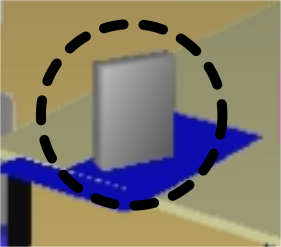
\includegraphics{cleantable/wait_for_pick}};
            \end{tikzpicture}
        };

        \node<1,5>[anchor=north] at (ph2 -| ahuman) (wait2) {%
            \begin{tikzpicture}
                \node[fill=white] (title) {\it wait for put\\ {\tt TAPE} \it into {\tt BIN}};
                \node[below=0.1 of title] {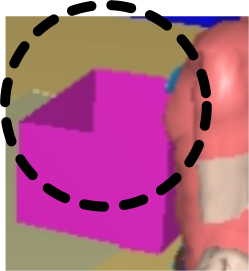
\includegraphics{cleantable/wait_for_throw}};
            \end{tikzpicture}
        };


        %%%%%%%%%%%%%%%%%%%%%%%%%%%%%%%%%%%%%%%%%%%%%%%%%%%%%%%%%%%%%%%%%%%%%%%%%%%%%%%%%%%%%%%%%%%%
        %%% FLOW
        %%%%%%%%%%%%%%%%%%%%%%%%%%%%%%%%%%%%%%%%%%%%%%%%%%%%%%%%%%%%%%%%%%%%%%%%%%%%%%%%%%%%%%%%%%%%
        \draw<1,2>[dotted, ->, in=45, out=180] (incoming.west) to (kb1);
        \draw<1,2>[dotted, ->, bend right] (kb1) to (pr1);
        \draw<1,2>[dotted, ->, bend left] (pr1) to (ep1);
        \draw<1,2>[dotted, ->, in=45, out=180] (ae1.west) to (kb2);
        \draw<1,3>[dotted, ->, bend right] (kb2) to (pr2);
        \draw<1,3>[dotted, ->, bend left] (pr2) to (ep2);
        \draw<1>[dotted, ->, in=45, out=180] (ae2.west) to (kb3);
        \draw<1,4>[dotted, ->, bend right] (kb3) to (ph1);
        \draw<1,4>[dotted, ->, bend left] (ph1) to (wait1);
        \draw<1>[dotted, ->, in=-20, out=180] (wait1.west) to (kb4.east);
        \draw<1,5>[dotted, ->, bend right] (kb4) to (ph2);
        \draw<1,5>[dotted, ->, bend left] (ph2) to (wait2);
        \draw<1,5>[dotted, ->, in=20, out=180] (wait2.west) to (kb5);
        \draw<1,5>[dotted, ->, bend left] (kb5.east) to (done.north);


 \end{tikzpicture}
 }
\end{frame}




%%%%%%%%%%%%%%%%%%%%%%%%%%%%%%%%%%%%%%%%%%%%%%%%%%%%%%%%

%\videoframe[0.56]{videos/dialogs.webm}
\videoframe[0.56]{videos/dialogs.webm?autostart}


\miniframesoff

\begin{frame}{}
    \begin{center}
        \Large
        That's all for today, folks!\\[2em]
        \normalsize
        Questions:\\
        \url{severin.lemaignan@brl.ac.uk} \\[1em]

        Slides:\\
        \href{https://github.com/severin-lemaignan/lecture-social-symbolic-reasoning}{\small
        github.com/severin-lemaignan/lecture-symbolic-reasoning}

    \end{center}
\end{frame}


\end{document}
